\documentclass[11pt]{article}
\usepackage[margin=1in]{geometry}
\usepackage[T1]{fontenc}
\usepackage{lmodern,microtype,amsmath,amssymb,amsthm,graphicx,booktabs,tabularx}
\usepackage{xcolor}
\usepackage{xurl}
\usepackage[colorlinks=true,allcolors=blue!45!black]{hyperref}
\usepackage{listings}
\usepackage{placeins}
\lstset{basicstyle=\ttfamily\small,breaklines=true,columns=fullflexible}
\renewcommand{\thesection}{S\arabic{section}}
\renewcommand{\thetable}{S\arabic{table}}
\renewcommand{\thefigure}{S\arabic{figure}}
\title{Supplementary Material 1\\\large Supplement to ``Pre-Export Row Scaling for Generated Mixed-Integer Programs: Accuracy Contracts and Software Evaluation''}
\author{Mathias Rodr\'iguez Castro\\\small Facultad de Ingenier\'ia, Universidad de la Rep\'ublica, Montevideo, Uruguay\\\small ORCID: \href{https://orcid.org/0009-0002-7235-7677}{0009-0002-7235-7677}\\\small\href{mailto:mathiasr@fing.edu.uy}{mathiasr@fing.edu.uy}}
\date{Prepared for Optimization Methods and Software}
\begin{document}
\maketitle
This supplement specifies the computational evidence and its limitations. Paths are
relative to the accompanying repository. Frozen results can be checked without an
optimizer license. The earlier draft and intermediate runs are retained to make
corrections traceable; they are not interchangeable with the final datasets.

\section{Proof for the triangular model}
For $R\in\mathbb R^{m\times n}$, $m,n\ge1$, set $\rho=\|R\|_2$ and
\[
 C_\gamma=\begin{bmatrix}I_n&0\\\gamma R&\gamma I_m\end{bmatrix},\qquad \gamma>0.
\]
The main-text proposition states that the unique optimal common coupling factor is
$(1+\rho^2)^{-1/2}$ and the minimum condition number is $\sqrt{1+\rho^2}+\rho$.
The interval-constrained optimum clips this factor to the interval.
\begin{proof}
An SVD of $R$ and orthogonal transformations reduce the nontrivial spectrum to
blocks $\left[\begin{smallmatrix}1&0\\\gamma\sigma&\gamma\end{smallmatrix}\right]$,
one for each singular value $\sigma$ of $R$, with possible additional singular
values $1$ or $\gamma$. Each block's squared singular values have product
$\gamma^2$ and sum $1+\gamma^2(1+\sigma^2)$. Their largest value increases and
smallest value decreases with $\sigma$; the block at $\sigma=\rho$ therefore
determines both extrema, including any additional values. If $k$ is their
singular-value ratio, then
\[
 k+k^{-1}=\frac{1+\gamma^2(1+\rho^2)}{\gamma}
 =\gamma^{-1}+\gamma(1+\rho^2).
\]
The left-hand side is increasing for $k\geq1$. The right-hand side has a unique
minimum at $\gamma_*=(1+\rho^2)^{-1/2}$, decreases before that point, and increases
after it. At the minimum, $k+k^{-1}=2\sqrt{1+\rho^2}$, whose root $k\geq1$ is
$\sqrt{1+\rho^2}+\rho$. The interval result follows from the same monotonicity.
For $\rho=0$, the argument reduces to balancing the diagonal entries at one.
\end{proof}

This scalar result assumes already whitened local blocks and one common coupling
factor. It does not solve general diagonal preconditioning and says nothing directly
about simplex bases or mixed-integer search.

\section{Fixed-basis conditioning audit}
\paragraph{Protocol.}
The protocol was fixed after a pilot on the first five inputs of each class
(\path{fixed-basis-recovery-20260914-v2/}) and then applied, unchanged except for the policy
set of the manuscript, to all 306 archived dispatch inputs with no exclusion: 204 Simple, 68
SG-Ter-Mer and 34 Full models. The audit build of the C++ generator writes five LP files per model through its
solver-free exporter, with the following preprocessing flags.
\begin{center}\small
\begin{tabular}{ll}
\toprule
Policy & Flags of \texttt{preprocesar}\\
\midrule
Base & \texttt{-{}-solodiagnostico}\\
Flat-GM & \texttt{-{}-local-matricial -{}-plano}\\
Flat-L2 & \texttt{-{}-local-matricial -{}-plano -{}-kernel-euclideo}\\
Role-Hybrid & \texttt{-{}-local-matricial -{}-acoplamiento-l2}\\
SA-Mat & \texttt{-{}-local-matricial}\\
\bottomrule
\end{tabular}
\end{center}
HiGHS 1.15.1 reads Base with small-matrix threshold $10^{-12}$, drops integrality and solves the
LP relaxation with the simplex method (one thread, random seed 0, 300-second limit); all 306
solves are optimal. The basis is stored by row and column names.

Each variant is read with the same reader and compared with Base before assembly: identical
named rows and columns, sparsity pattern, bounds, objective, offset and integrality. A row's
factor is inferred from its largest-magnitude coefficient, and the whole row and both RHS values
must agree with that factor to relative tolerance $2\times10^{-13}$; the largest observed
deviation is $2.5\times10^{-16}$. The basis consists of the basic structural columns of the
variant's own matrix and a unit column for every basic slack.

\paragraph{Estimate and verification.}
$\|B\|_1$ is computed from the stored entries, and $\|B^{-1}\|_1$ is estimated by SciPy's
\texttt{onenormest} ($t=4$) on solves with a SuperLU factorization, with seeds 0, 1 and 2; the
tables use seed 0. The seeds agree within a factor of 2.4, and 63 of 1,530 records differ by more
than 1\%. The largest componentwise backward error of a diagnostic solve is $1.9\times10^{-8}$.
The script \path{scripts/research/verify_fixed_basis.py} imports neither the driver nor the
HiGHS reader. It checks the recorded hashes, parses every LP file as text, rebuilds each basis
from the stored names and compares it entry by entry with the stored matrix: all 1,530 bases
match exactly. It then recomputes each estimate as $B^{-1}=Q^{-1}D$, with $Q=DB$ and $D$ an exact
power-of-two row equilibration. The two routes differ by less than $10^{-6}$ in 1,512 records and
by at most 23\% in all; since their test solutions agree to $10^{-12}$ in every record, the
remaining differences point to the randomized estimator's iteration path rather than to the
solves.

\begin{table}[tb]
\centering\small
\caption{Fixed-basis audit: per-instance ratios $\kappa_1(\text{policy})/\kappa_1(\text{Base})$ on
the common basis. ``Improved'' counts ratios below one.}\label{tab:si-fixed-basis}
\begin{tabular}{llrrrrr}
\toprule
Class & Policy & $n$ & Median ratio & Minimum & Maximum & Improved \\
\midrule
Simple & Flat-GM & 204 & $2.4\times10^{-7}$ & $1.9\times10^{-8}$ & $1.7\times10^{-3}$ & 204 \\
Simple & Flat-L2 & 204 & 1.57 & $3.3\times10^{-4}$ & $2.7\times10^{2}$ & 32 \\
Simple & Role-Hybrid & 204 & $2.4\times10^{-7}$ & $1.9\times10^{-8}$ & $1.7\times10^{-3}$ & 204 \\
Simple & SA-Mat & 204 & $2.4\times10^{-7}$ & $1.9\times10^{-8}$ & $1.7\times10^{-3}$ & 204 \\
\addlinespace
SG-Ter-Mer & Flat-GM & 68 & $7.3\times10^{-9}$ & $1.5\times10^{-9}$ & $1.2\times10^{-2}$ & 68 \\
SG-Ter-Mer & Flat-L2 & 68 & 1.51 & $8.1\times10^{-4}$ & 18.61 & 10 \\
SG-Ter-Mer & Role-Hybrid & 68 & $7.3\times10^{-9}$ & $1.5\times10^{-9}$ & 0.57 & 68 \\
SG-Ter-Mer & SA-Mat & 68 & $7.3\times10^{-9}$ & $1.5\times10^{-9}$ & 0.57 & 68 \\
\addlinespace
Full & Flat-GM & 34 & $3.5\times10^{-7}$ & $9.3\times10^{-9}$ & $3.1\times10^{-6}$ & 34 \\
Full & Flat-L2 & 34 & 1.49 & 0.85 & $1.5\times10^{2}$ & 2 \\
Full & Role-Hybrid & 34 & $3.5\times10^{-7}$ & $9.3\times10^{-9}$ & $3.1\times10^{-6}$ & 34 \\
Full & SA-Mat & 34 & $3.5\times10^{-7}$ & $9.3\times10^{-9}$ & $3.1\times10^{-6}$ & 34 \\
\bottomrule
\end{tabular}

\end{table}

\paragraph{Interpretation.}
Row scaling changes $\kappa_1$, so the audit measures the exported representation before any
solver-internal scaling. The Base estimates exceed the reciprocal of machine precision; the
precision check below shows that they are nevertheless accurate on a stress sample. Every row of the 306 models has a coefficient of magnitude at
least one, and $1/\|a_r\|_2\le1/\max_j|a_{rj}|$, so no Flat-L2 factor exceeds one. Across all
rows, Flat-GM enlarges 22.5\% (Simple), 32.1\% (SG-Ter-Mer) and 27.3\% (Full) and leaves 30.0\%,
22.0\% and 24.5\% unscaled; Flat-L2 enlarges none and leaves 57.6\%, 64.3\% and 59.2\% unscaled.
SA-Mat and Role-Hybrid exports are byte-identical on all 306 models. SA-Mat coincides with
Flat-GM on every Simple model and, in each SG-Ter-Mer and Full model, differs from it only on
the 1,440 \texttt{falla\_tramo} market-shortage rows, which SA-Mat and Role-Hybrid leave
unscaled. The authoritative directory is
\path{results-revision/research-audit/fixed-basis-final-20260914/}, with design, source
snapshot, exports, bases, per-row factors, verification and \texttt{analysis.json}.

\paragraph{Precision check.}
Because the unscaled values exceed the reciprocal of machine precision, the script
\path{scripts/research/verify_fixed_basis_precision.py} checks their accuracy on a stress sample
fixed before computation: in each class, the model with the largest Base estimate, the model with
the largest Flat-GM/Base estimated ratio, and one other model drawn with seed 20260915. In Full
the first two coincide (instance014), which gives eight models and 24 bases under Base, Flat-GM
and Flat-L2. For each hash-checked basis, $\|B\|_1$ is computed in exact rational arithmetic.
Every column of $B^{-1}$ is solved in double precision; with $x_j$ the computed column and
$\rho_j$ a bound on $\|Bx_j-e_j\|_1$ that includes the rounding-error terms of the residual
evaluation, $\|B^{-1}\|_1\le\max_j\|x_j\|_1/(1-\max_j\rho_j)$ whenever $\max_j\rho_j<1$. This
upper endpoint is evaluated in floating point with explicit error terms rather than directed
rounding; the implementation does not provide a formal rounding certificate for that
endpoint. We therefore call the resulting ranges diagnostic brackets, not certified
enclosures. For the five largest columns, the solution is refined with residuals computed exactly
in rational arithmetic on the stored binary64 data; since $\|B^{-1}\|_1\ge\|x\|_1/\|Bx\|_1$ for
every nonzero $x$, the exact quotient certifies a lower bound.

The largest residual bound is $6.0\times10^{-3}$, and refinement stops within two steps. The
diagnostic brackets have relative width at most $6.0\times10^{-3}$ for Base, $4.8\times10^{-3}$ for
Flat-L2 and $2.0\times10^{-5}$ for Flat-GM, and the computed upper estimate of the Flat-GM/Base ratio
agrees with the estimated ratio to $2.1\times10^{-5}$ in all eight models
(Table~\ref{tab:si-precision}). Twenty-three of the 24 estimates lie inside their brackets. The
Flat-L2 estimate for Full instance046 is 2.4 times smaller than its certified lower bound, as a
lower-bound estimator can be; this makes Flat-L2 less favorable, not more. Outputs are in
\path{precision-check/} within the audit directory.

\begin{table}[tb]
\centering\small
\caption{Precision check on the stress sample. ``Base $\kappa_1\ge$'' is the certified lower
bound. ``Bracket width'' is the largest relative width (computed upper endpoint over lower bound, minus one)
among Base, Flat-GM and Flat-L2. The last two columns give the estimated ratio
$\kappa_1(\text{Flat-GM})/\kappa_1(\text{Base})$ and its upper estimate, the floating-point upper
endpoint for Flat-GM divided by the certified lower bound for Base. Only the lower
bounds carry the rational certification described above.}\label{tab:si-precision}
\begin{tabular}{llrrrr}
\toprule
Class & Model & Base $\kappa_1\ge$ & Bracket width & Flat-GM/Base estimate & Upper estimate \\
\midrule
Simple & caso32e & $9.3\times10^{19}$ & $1.5\times10^{-4}$ & $2.405\times10^{-6}$ & $2.405\times10^{-6}$ \\
Simple & caso05f & $1.0\times10^{19}$ & $3.7\times10^{-3}$ & $1.681\times10^{-3}$ & $1.681\times10^{-3}$ \\
Simple & caso27f & $8.7\times10^{18}$ & $1.9\times10^{-5}$ & $1.077\times10^{-7}$ & $1.077\times10^{-7}$ \\
SG-Ter-Mer & instance067 & $1.2\times10^{21}$ & $4.1\times10^{-3}$ & $6.247\times10^{-6}$ & $6.247\times10^{-6}$ \\
SG-Ter-Mer & instance028 & $4.0\times10^{11}$ & $1.5\times10^{-6}$ & $1.216\times10^{-2}$ & $1.216\times10^{-2}$ \\
SG-Ter-Mer & instance074 & $4.0\times10^{20}$ & $9.5\times10^{-5}$ & $2.277\times10^{-9}$ & $2.277\times10^{-9}$ \\
Full & instance014 & $1.2\times10^{22}$ & $6.0\times10^{-3}$ & $3.055\times10^{-6}$ & $3.055\times10^{-6}$ \\
Full & instance046 & $4.7\times10^{20}$ & $2.7\times10^{-4}$ & $6.046\times10^{-7}$ & $6.046\times10^{-7}$ \\
\bottomrule
\end{tabular}

\end{table}

\paragraph{Archived fixed-incumbent computation.}
An earlier computation (\path{results-revision/fixed-basis/}) used a different reference
basis: Gurobi solved each Base MIP (relative gap $10^{-3}$, 16 threads), fixed the integers at its
incumbent and took the basis of the resulting LP. Its archived medians point in the same
direction with smaller magnitudes; for SA-Mat relative to Base they are $1.2\times10^{-3}$
(Simple), $3.6\times10^{-4}$ (Full) and 0.41 (SG-Ter-Mer). The magnitudes therefore depend on the
reference basis. That computation did not retain its exports, basis identities or binary hash,
and its multithreaded incumbents cannot be replayed, so it is not used as evidence. The
provenance audit is in \path{results-revision/research-audit/fixed-basis-recovery-20260914-v2/}.

\section{Computing environment}
Table~\ref{tab:environment} separates the historical experiments from the local OMS
campaigns. The historical operational PAR10, local Ruiz comparison and full-process
measurements in Tables~S15--S16 use wall seconds. These depend on hardware and load;
the local timings describe the measured prototype on a shared machine. The 144-call
comparison also spans a documented reboot. Native Work and deterministic ticks are
reported within their respective solver/version, without equating them with wall time
or with each other.

All 240 historical operational logs identify the same processor and operating system.
The laptop logs in \path{operational/precision-smoke/} belong to a separate test.
The two historical replications used ClusterUY/SLURM with 16 cores per task; their
node models were not recorded. Historical fixed-basis, matrix and stress machine
identities remain unrecorded. The newer dispatch logs identify an Intel i7-13620H
running Ubuntu 22.04.5 LTS. Original records, not the current host, supply these identities.

\begin{table}[tb]
\centering\footnotesize
\caption{Computing environment by campaign. Missing historical machine identities
are not reconstructed. Local wall times depend on the shared-machine load; offline
reference LP settings are stated in the corresponding protocols.}
\label{tab:environment}
\resizebox{\textwidth}{!}{\begin{tabular}{llllll}
\toprule
Campaign & Optimizer & Thr. & Limit & Machine & Reported quantity \\
\midrule
\multicolumn{6}{l}{\emph{Historical experiments}}\\
Fixed-basis audit    & HiGHS 1.15.1 (LP only)       & 1  & 300~s   & not recorded              & $\kappa_1$ \\
Matrix audit         & none                         & --- & ---    & not recorded              & $\kappa_2^{+}$, identity \\
Operational campaign & Gurobi 13.0.1                & 16 & 1,800~s & Xeon Gold 6138, Debian 12 & PAR10 (s), work units \\
Replication, seed 7  & Gurobi 13.0.1                & 16 & 1,800~s & ClusterUY, node not recorded & work units \\
Replication, CPLEX   & CPLEX 22.1.2.0               & 16 & 1,800~s & ClusterUY, node not recorded & deterministic ticks \\
Stress experiment    & HiGHS 1.15.1, Gurobi 13.0.2, & 1  & 10~s    & not recorded              & verified counts \\
                     & CPLEX 22.1.2.0               &    &         &                           & \\
\midrule
\multicolumn{6}{l}{\emph{Local OMS campaigns: Intel i7-13620H, Ubuntu 22.04.5 LTS}}\\
Ruiz/stage comparison & Gurobi 13.0.2 & 4 & 120~s & shared local machine & Work, PAR10 (s)\\
Activation follow-up & Gurobi 13.0.2 & 4 & 120~s & shared local machine & budgets, Work\\
Common-incumbent control & Gurobi 13.0.2 & 4 & 12~s / 12 Work & shared local machine & Work, counts\\
Matched IF control & Gurobi 13.0.2 & 4 & 120~s & shared local machine & Work, total (s)\\
Matched accuracy/remedies & Gurobi 13.0.2 & 4 & 120~s & shared local; reboot retained & Work, total (s)\\
\bottomrule
\end{tabular}
}
\end{table}

\section{Operational evidence and reconstruction}
The final historical campaign assigned 15 instances in each of two dispatch families,
four policies, and two relative MIP gaps. Thus there are 240 assigned Gurobi 13.0.1 runs (Table~\ref{tab:environment}).
All use seed 42, 16 threads and a 1,800-second limit. The four policies are Base,
Flat-GM, Flat-L2 and Role-Hybrid. The assigned instances are

\begin{quote}\small\raggedright
Simple: \path{caso01a}, \path{caso03b}, \path{caso05d}, \path{caso10e}, \path{caso14a}, \path{caso20c}, \path{caso22d}, \path{caso24f}, \path{caso27a}, \path{caso29c}, \path{caso31e}, \path{caso33f}, \path{caso42b}, \path{caso44c}, \path{caso46e}.\\[2pt]
SG-Ter-Mer: \path{instance001}, \path{instance005}, \path{instance014}, \path{instance022}, \path{instance027}, \path{instance031}, \path{instance042}, \path{instance046}, \path{instance051}, \path{instance058}, \path{instance068}, \path{instance072}, \path{instance077}, \path{instance081}, \path{instance092}.
\end{quote}

\noindent They are those of the historical campaign and are spread across the ordering of each
class, but the rule that produced them was not recorded, so this is a description of the subsets
rather than evidence of a pre-registered design. What can be checked is that they predate the
analysis: the runs are reconstructed from logs retrieved from the cluster, and the frozen tables
of the two replications reuse the same two lists. The analysis retains the assigned subsets and
includes every non-completion in the primary runtime endpoint.

For assigned instance $i$ in a cell, let $t_i$ be the recorded runtime and define
$T_i=t_i$ for completion and $T_i=18{,}000$ otherwise. The primary summary is
$15^{-1}\sum_i T_i$. This PAR10 endpoint measures operational completion under
the specified stopping criteria. It is not an exact primal or optimality certificate.
In particular, a solver-completed point with a concerning original residual is still
counted as completed, with feasibility diagnostics reported separately.

\paragraph{Scenario defect in the SG-Ter-Mer instances.}
The market dispatch of this family reads a local demand series and a total demand series. In
the historical instances the total series was rebuilt from a noisy rescaling of residual
demand, and in 39 of the 68 instances it falls below the local demand in at least one hour: 9
of the 15 instances assigned above, among them instance077, where the inversion occurs in 22
hours and reaches 259 units. The exported models remain well-posed MILPs and every comparison
in this paper is between representations of the same model, so no reported equivalence,
residual or effort measurement is affected. What the defect does mean is that those instances
are not faithful market scenarios and that the physical reading of their solutions is
unreliable. A corrected version of the family, rebuilt from the authoritative demand series,
exists outside this work and shows no inversion; no result reported here uses it. The counts
above are produced by \path{scripts/research/check_sgtm_demand.py} from the instance files in
the archive.

\paragraph{Does the defect drive the SG-Ter-Mer result?}
Six of the fifteen instances are free of the inversion. Table~\ref{tab:defect-sensitivity} repeats
the two endpoints on that subset, with the same work measure and the same common-completion
pool as the main text. The conditional gain does not depend on the defective scenarios: the
Flat-GM work ratio is 0.452 at a 1\% gap and 0.502 at 0.1\% on the six, against 0.698 and 0.682
on all fifteen. The failure-sensitive reversal does depend on them, for a reason worth stating:
the instance that times out under every scaled policy, instance077, is one of the nine, so on
the defect-free subset every scaled policy completes and PAR10 follows the conditional gain
instead of contradicting it. The reversal reported in the main text therefore rests on a single
instance, which is what makes it a statement about failure sensitivity rather than about
typical effort.

\begin{table}[tb]
\centering\small
\caption{SG-Ter-Mer reconstruction on all fifteen assigned instances and on the six without the
demand inversion. Work ratios are geometric means against Base on the instances every policy
completed; PAR10 is the arithmetic mean over the assigned pool, with 18,000 seconds for a
non-completion.}
\label{tab:defect-sensitivity}
\begin{tabular}{llrrrr}
\toprule
& & \multicolumn{2}{c}{Work ratio vs Base} & \multicolumn{2}{c}{Mean PAR10 (s)} \\
Gap & Policy & All 15 & Defect-free 6 & All 15 & Defect-free 6 \\
\midrule
1\% & Base & --- & --- & 116.2 & 22.8 \\
 & Flat-GM & 0.698 & 0.452 & 1216.5 & 5.9 \\
 & Flat-L2 & 0.863 & 0.844 & 1217.6 & 14.4 \\
 & Role-Hybrid & 0.745 & 0.470 & 1217.3 & 5.4 \\
\addlinespace
0.1\% & Base & --- & --- & 134.1 & 25.0 \\
 & Flat-GM & 0.682 & 0.502 & 1216.2 & 7.1 \\
 & Flat-L2 & 0.802 & 0.838 & 1216.0 & 13.6 \\
 & Role-Hybrid & 0.726 & 0.493 & 1216.9 & 6.2 \\
\bottomrule
\end{tabular}

\end{table}

\paragraph{Work and uncertainty.}
The old runner's scaled-policy Work markers inherited a fixed, zero-decimal stream
format. Native Gurobi summaries instead retain two decimals. The reconstruction uses
those native summaries for every policy, at their common 0.01-unit resolution. It
never combines a Work value with a timeout penalty measured in seconds. Byte equality
of rounded Work or node counts cannot prove equality of exported models.

Secondary Work ratios use only the instances completed by every policy in a given
family/gap cell. Ratios are paired by instance; their geometric mean is
$\exp(n^{-1}\sum_i\log(W_{i,p}/W_{i,\mathrm{Base}}))$. Percentile intervals use
10,000 paired bootstrap samples, seed 20260908. These are exploratory intervals,
without multiplicity adjustment, and are conditional on the common completion pool.
A separate sensitivity calculation uses the intervals of width 0.01 implied by
rounding each native Work value. Neither calculation accounts for the excluded
timeout's unobserved completion effort.

Flat-GM/Base on the 14 common completed SG-Ter-Mer instances has ratios 0.698
with interval $[0.486,0.944]$ at 1\% gap, and 0.682 with $[0.470,0.925]$ at
0.1\%. However, instance077 completes under Base and times out under all three
scaled policies at both gaps. For Simple at 1\%, Flat-L2/Base has Work ratio 1.792
with interval $[1.033,3.542]$. These conditional observations do not establish a
uniform solver advantage. Table~\ref{tab:si-operational} gives the complete PAR10 summary.

\begin{table}[tb]
\centering\small
\caption{Reconstructed operational campaign. Arithmetic mean PAR10 in seconds on the
15 assigned instances per cell; a timeout contributes 18,000 seconds. Parentheses give
completed runs. All rows concern Gurobi.}\label{tab:si-operational}
\begin{tabular}{llrrrr}
\toprule
Class & Gap & Base & Flat-GM & Flat-L2 & Role-Hybrid \\
\midrule
Simple & 1\% & 11.90 (15) & 2.12 (15) & 20.44 (15) & 2.11 (15) \\
Simple & 0.1\% & 52.00 (15) & 72.98 (15) & 33.17 (15) & 72.63 (15) \\
SG-Ter-Mer & 1\% & 116.15 (15) & 1216.51 (14) & 1217.60 (14) & 1217.34 (14) \\
SG-Ter-Mer & 0.1\% & 134.08 (15) & 1216.24 (14) & 1216.05 (14) & 1216.91 (14) \\
\bottomrule
\end{tabular}
% Entries: arithmetic mean PAR10 in seconds (number completed out of 15).
% Time limit: 1800 seconds; every non-completion receives 18000 seconds.
% These are exploratory single-seed, fixed-pool observations, not a superiority test.

\end{table}

\paragraph{Replication under a second seed and a second solver.}
The reconstruction fixes the solver, the seed and the thread count. To separate what is stable
from what belongs to that configuration, the same 30 instances, four policies, two gaps,
1,800-second limit and 16 threads were rerun twice, changing one factor at a time: Gurobi with
seed 7, and CPLEX with the original seed 42. The run tables were frozen before the runs, the
policy order within an instance is seeded by the instance digest, and the records carry the same
verification as the campaign. Table~\ref{tab:replication} reports the paired effort ratio
against Base on the instances every policy completed. Effort is each solver's own measure, work
units for Gurobi and deterministic ticks for CPLEX, so a column is read within its solver and
never across. Runs classified as infrastructure failures were repeated and solver timeouts were not; there were two such
episodes, the eight Gurobi runs of one instance that failed while the licence server was
saturated, and the eight CPLEX runs of instance077, repeated with more memory after one of them
was killed by the cgroup limit. The instance that reverses the PAR10 ordering in the reconstruction,
instance077, behaves differently in every condition: under Gurobi at seed 7 all
eight of its runs reach the limit, Base included, while under CPLEX the run that reaches the
limit is Base at the 1\% gap and Role-Hybrid at 0.1\%.

\begin{table}[tb]
\centering\small
\caption{Paired effort ratio against Base on the instances completed by every policy, with
bootstrap intervals, for the reconstruction and its two replications. Values below one favour
the scaled policy.}
\label{tab:replication}
\begin{tabular}{llrrr}
\toprule
& & Gurobi, seed 42 & Gurobi, seed 7 & CPLEX, seed 42 \\
\midrule
\multicolumn{5}{l}{\emph{Simple, gap 1\%}} \\
\quad Flat-GM & & 0.631 [0.31, 1.03] & 0.783 [0.47, 1.03] & 0.609 [0.28, 1.04] \\
\quad Flat-L2 & & 1.792 [1.03, 3.54] & 2.226 [1.16, 4.70] & 1.306 [0.39, 4.26] \\
\quad Role-Hybrid & & 0.631 [0.31, 1.03] & 0.783 [0.47, 1.04] & 0.609 [0.28, 1.04] \\
\addlinespace
\multicolumn{5}{l}{\emph{Simple, gap 0.1\%}} \\
\quad Flat-GM & & 1.063 [0.89, 1.25] & 1.002 [0.91, 1.10] & 0.837 [0.53, 1.15] \\
\quad Flat-L2 & & 1.385 [0.90, 2.33] & 1.524 [1.05, 2.41] & 1.425 [0.52, 3.64] \\
\quad Role-Hybrid & & 1.063 [0.89, 1.24] & 1.002 [0.91, 1.10] & 0.837 [0.53, 1.14] \\
\addlinespace
\multicolumn{5}{l}{\emph{SG-Ter-Mer, gap 1\%}} \\
\quad Flat-GM & & 0.698 [0.49, 0.94] & 0.743 [0.49, 1.02] & 1.078 [0.99, 1.18] \\
\quad Flat-L2 & & 0.863 [0.72, 1.03] & 1.135 [0.92, 1.42] & 0.955 [0.92, 0.99] \\
\quad Role-Hybrid & & 0.744 [0.49, 1.04] & 0.751 [0.48, 1.03] & 1.053 [0.98, 1.15] \\
\addlinespace
\multicolumn{5}{l}{\emph{SG-Ter-Mer, gap 0.1\%}} \\
\quad Flat-GM & & 0.682 [0.47, 0.92] & 0.745 [0.49, 1.03] & 1.077 [0.99, 1.18] \\
\quad Flat-L2 & & 0.802 [0.65, 0.98] & 1.134 [0.94, 1.39] & 0.994 [0.93, 1.09] \\
\quad Role-Hybrid & & 0.726 [0.48, 1.00] & 0.759 [0.49, 1.04] & 1.052 [0.97, 1.16] \\
\bottomrule
\end{tabular}

\end{table}

\paragraph{Original residual normalization.}
For an equality, the absolute residual is $|a_r^Tx-b_r|$. The RHS-normalized
residual divides by $1+|b_r|$, whereas the activity-normalized residual divides by
$\max\{1,|b_r|,\sum_j|a_{rj}x_j|\}$. For inequalities the positive violation replaces the
absolute equality residual. Neither is a supplied engineering acceptance budget.
For caso46e, Flat-L2 at 1\% produces an absolute equality residual about 4.97 on
a row with zero RHS. Its RHS-normalized value is still 4.97, while the run's maximum
activity-normalized residual is $1.15\times10^{-7}$. Calling the former a 497\%
physical error would be unjustified.

The directory \path{results-revision/research-audit/operational/} contains native
cluster logs, the reconstructed run table, cell summaries, paired contrasts, original
input hashes and analysis settings. The script
\path{scripts/audit_operational_evidence.py} generates these summaries and the
main-text table. A separate two-run smoke check under \path{precision-smoke/}
verifies that the corrected C++ Work marker preserves the solver API's precision;
it does not replace any of the 240 historical observations.

\paragraph{Historical stage ablation.}
The earlier preprocessing campaign included a stage ablation under Gurobi. It predates the
attribution analysis of the present article and is reported here only as exploratory evidence
about solver effort. The structured rules had three conceptual stages: local-row normalization,
block-scale construction and coupling-row scaling. The ablation retained either the local stage
alone or the coupling stage alone and compared them with Base and the full rule on the same
instance banks, at relative MIP gaps of 1\% and 0.1\%.

Table~\ref{tab:stage-ablation} gives the structured rule on all three classes. Local-only
normalization reproduces the full rule's shifted geometric mean of solver time in every cell,
to within 0.5\% except on Simple at a 1\% gap, where the two differ by 0.01~s. Coupling-only
scaling never improves on Base: it matches it on Simple and SG-Ter-Mer and is 1 to 2\% above it
on Full. The matrix rule, recorded in the same files, agrees cell by cell with one exception
worth stating: on Full at a 0.1\% gap it does not improve on Base at all (396.71~s for the full
rule against 373.58~s), and local-only tracks it there as elsewhere (394.67~s). The attribution
is therefore about where a stage-wise difference sits, not a claim that either rule always helps.

This does not contradict the coupling-kernel attribution of the article. That concerns which
kernel explains a representation-level conditioning difference under matched controls; this
ablation concerns where an operational Gurobi time difference arose in an earlier campaign. The
endpoints and the comparisons are different.

\begin{table}[htb]
\centering\small
\caption{Historical stage ablation, structured rule. Shifted geometric mean of solver time in
seconds, Gurobi. The ablation belongs to the earlier preprocessing campaign and is not a rerun
of the present policy set; \texttt{make research-stage-ablation} recomputes it from the stored
runs in \texttt{results-revision/r5-ablation/}.}
\label{tab:stage-ablation}
\begin{tabular}{llrrrrr}
\toprule
Class & Gap & $n$ & Base & Full rule & Local only & Coupling only \\
\midrule
Simple & 1\% & 204 & 3.73 & 2.02 & 2.01 & 3.74 \\
Simple & 0.1\% & 204 & 9.61 & 6.41 & 6.39 & 9.59 \\
SG-Ter-Mer & 1\% & 68 & 14.42 & 8.55 & 8.58 & 14.45 \\
SG-Ter-Mer & 0.1\% & 68 & 16.15 & 9.79 & 9.76 & 16.16 \\
Full & 1\% & 34 & 82.55 & 71.41 & 70.94 & 83.69 \\
Full & 0.1\% & 34 & 373.58 & 325.73 & 325.91 & 376.29 \\
\bottomrule
\end{tabular}

\end{table}

\section{Fresh matrix audit}
Ten seeds, 20260909--20260918, are crossed with exponent ranges $[-R,R]$ for
$R\in\{1,2,3\}$, two disturbance severities (3 and 6), and three coupling patterns:
\texttt{coupling}, \texttt{coupling\_uniform}, and \texttt{mixed}. There are 180
instances and six exports per instance: Base, SA-Mat, Flat-GM, Flat-L2, Role-Hybrid
and SA-Mat-permB. A solver-free DummyLp backend writes the 1,080 LP files.

The parser compares named rows and columns, coefficient supports, row senses,
right-hand sides, and the remaining objective/domain sections. It infers each row's
positive factor from a nonzero pivot coefficient and checks the entire row and RHS
at relative tolerance $10^{-13}$. All final exports pass. This remains a
floating-point proportionality check; it is not a rational proof of exact scaling.
Byte hashes supply the stronger literal-identity claims where they hold.

The numerical reference rank is determined from row-L2-normalized Base using a
relative threshold $10^{-12}$. Every variant then uses that same rank for the
spectral diagnostic. Independent rank thresholds on each export disagree on 25 of
1,080 cases. Very large unscaled condition estimates near binary64 resolution are
therefore not interpreted quantitatively. The paired scaled diagnostics are below
$6.5\times10^6$.

The authoritative directory is
\path{results-revision/research-audit/identifiability-final/}. Its manifest records
the generator binary and script hashes, settings, named comparisons and all exports.
The retained \texttt{identifiability-confirmatory/} directory used the former fixed
precision serializer and is superseded for current matrix claims.

\section{Frozen binary stress protocol}
The experiment crosses three binary families, eight seeds (100--107), and four
coefficient exponents (0, 3, 6, 9): 96 models with 12 binary variables each. Each
model is run under two presolve settings, three solvers, and nine policies, giving
5,184 planned configurations. Budget-round abstains on 432 configurations before
calling an optimizer; hence there are 4,752 actual calls. These configurations are
not statistically independent observations.

For seed $s$, NumPy's default generator is seeded by $20260908+s$. The cardinality
family has one all-ones row. Packing uses three rows of uniformly sampled integers
1 through 9. Signed rows use integers from $-9$ through 9, replacing zeros by one.
For row $r$, $k_r=\max\{2,\lfloor0.55\sum_j\max(W_{rj},0)\rfloor\}$; profits
are uniform integers 1 through 30. The represented constraints are
$10^e Wx\le10^e k-0.1\boldsymbol1$. Integer enumeration proves the binary optimum
for each stored model. Changing $e$ also changes the relaxation; it is not pure
row re-emission. The budget is 0.01 in the declared canonical stress-test units.

All three solvers use one thread, the instance seed, a ten-second limit and zero target
absolute and relative MIP gaps. Primal and integrality tolerances are $10^{-6}$,
except GM-tight, which uses $10^{-9}$. Gurobi's enabled-presolve arm uses its automatic
presolve setting; HiGHS uses presolve on. Internal solver scaling remains at its
default. Recorded versions are Python 3.10.12, NumPy 2.2.6, HiGHS 1.15.1 and
Gurobi 13.0.2. Solving uses the Python APIs rather than text-file import.

Base, GM and L2 scale all rows according to their stated kernels, without a skip
band. Budget-only uses $\epsilon/\delta_r$. Budget-GM projects GM onto the joint
budget/coefficient interval with window $[10^{-9},10^9]$. Budget-round additionally
reserves $10^{-6}\sum_j|a_{rj}|$ for rounding and rejects the whole model if any
row's contract is incompatible. Dyadic-GM imposes the coefficient window and exact
binary64 multiplication, including the RHS; Budget-dyadic also imposes the residual
budget. The latter two policies were added after the initial floating-endpoint audit
and are exploratory, not a new holdout experiment.

The sequence of preserved datasets under
\path{results-revision/research-audit/} is:
\begin{center}\small
\begin{tabularx}{\linewidth}{lX}
\toprule
Directory & Interpretation\\
\midrule
\texttt{budget-pilot} & Single exploratory seed 0; six initial policies.\\
\texttt{budget-confirmatory} & Seeds 100--107; seven policies; original nearest-rounded endpoint.\\
\texttt{budget-confirmatory-v2} & Same seven policies and seeds; exact endpoints rounded inward.\\
\texttt{budget-final} & Authoritative nine-policy run; inward endpoints and two exploratory dyadic controls.\\
\bottomrule
\end{tabularx}
\end{center}
An attractive result from an intermediate implementation is not substituted for the
corrected final result. In particular, the earlier HiGHS Budget-GM count of 191
verified configurations becomes 182 with correctly inward-rounded endpoints.

\begin{table}[tb]
\centering\small
\caption{Enumerated stress experiment, 192 planned configurations per policy and solver.
``Verified'' means that the returned point passes the declared acceptance rule and its
rounded assignment attains the independently enumerated optimum. ``Other'' includes
unverified outputs and solver errors; ``Abstain'' means no optimizer call was attempted.
Abstention is not a performance success. The separated GCD-floor row is the later
integer-aware control, with the same denominator and acceptance rule.}\label{tab:budget-results}
\begin{tabular}{lrrrrrrrrr}
\toprule
& \multicolumn{3}{c}{HiGHS 1.15.1} & \multicolumn{3}{c}{Gurobi 13.0.2} & \multicolumn{3}{c}{CPLEX 22.1.2} \\
Method & Verified & Other & Abstain & Verified & Other & Abstain & Verified & Other & Abstain \\
\midrule
Base & 167 & 25 & 0 & 156 & 36 & 0 & 150 & 42 & 0 \\
GM & 141 & 51 & 0 & 140 & 52 & 0 & 140 & 52 & 0 \\
L2 & 141 & 51 & 0 & 139 & 53 & 0 & 140 & 52 & 0 \\
GM-tight & 166 & 26 & 0 & 166 & 26 & 0 & 166 & 26 & 0 \\
Dyadic-GM & 142 & 50 & 0 & 140 & 52 & 0 & 140 & 52 & 0 \\
Budget-only & 191 & 1 & 0 & 151 & 41 & 0 & 140 & 52 & 0 \\
Budget-GM & 182 & 10 & 0 & 152 & 40 & 0 & 140 & 52 & 0 \\
Budget-dyadic & 161 & 31 & 0 & 153 & 39 & 0 & 140 & 52 & 0 \\
Budget-round & 48 & 0 & 144 & 48 & 0 & 144 & 48 & 0 & 144 \\
\midrule
GCD-floor & 192 & 0 & 0 & 192 & 0 & 0 & 192 & 0 & 0 \\
\bottomrule
\end{tabular}

\end{table}

\paragraph{Paired outcomes and factor distances.}
The paired comparison in the main text uses identical model, presolve and solver keys; its
counts are regenerated by \path{scripts/research/analyze_budget_experiment.py}, which also writes
\path{budget-final/paired-discordance.json}. Budget-only and Budget-GM select different factors at
multipliers $10^0$ and $10^3$, where both verify every configuration on all three solvers. At $10^6$
and $10^9$ the budget endpoint binds, and Budget-GM returns the inward-rounded endpoint, at most
one unit in the last place from Budget-only's factor $\epsilon/\delta$ on every row of every
model. All ten configurations whose verification outcomes differ between the two policies lie at
these multipliers. The failure categories quoted in the main text are taken from
\path{results-revision/research-audit/exploration-failures/summary.json} for HiGHS and Gurobi and
\path{exploration-failures-cplex/summary.json} for CPLEX, both written by the same script, which
classifies each returned point with an infeasible rounded assignment by whether it violates the
original row budget and whether it violates the exported tolerance.

\paragraph{Classical integer-row controls.}
The follow-up in \path{results-revision/research-audit/exploration-lattice/}
uses the same 96 stored models, three solvers and two presolve settings. For an
integral row $a^Tz\le b$, let $g=\gcd_j |a_j|$ and replace it by
$(a/g)^Tz\le\lfloor b/g\rfloor$. Exact rational division of the stored RHS
determines the floor. GCD-floor exports this row directly; GCD-floor-GM adds
floating GM normalization; GCD-midgap-GM first replaces the floored RHS by
$\lfloor b/g\rfloor+1/2$ and then applies GM. The three controls account for
1,728 further calls, all yielding verified original-model optima. The midpoint
operation is integer-equivalent before multiplication and weakens the LP relative
to flooring. These are established reductions or arithmetic controls, not new
scaling proposals.

The direct GCD-floor export preserves all 96 binary feasible sets exactly and
verifies 192/192 configurations per solver. Independent enumeration of the
actual binary64 exports also finds equivalence for all 96 GCD-midgap-GM models,
but detects excluded feasible boundary points in 60 of the GCD-floor-GM models.
Thus successful returned optima do not establish equivalence of every represented
constraint. The main comparison foregrounds GCD-floor, whose transformation and
export are both exact for these inputs. This arithmetic distinction also explains
why an exact-export condition is separate from selecting a mathematically
admissible real factor.

\begin{figure}[tb]
\centering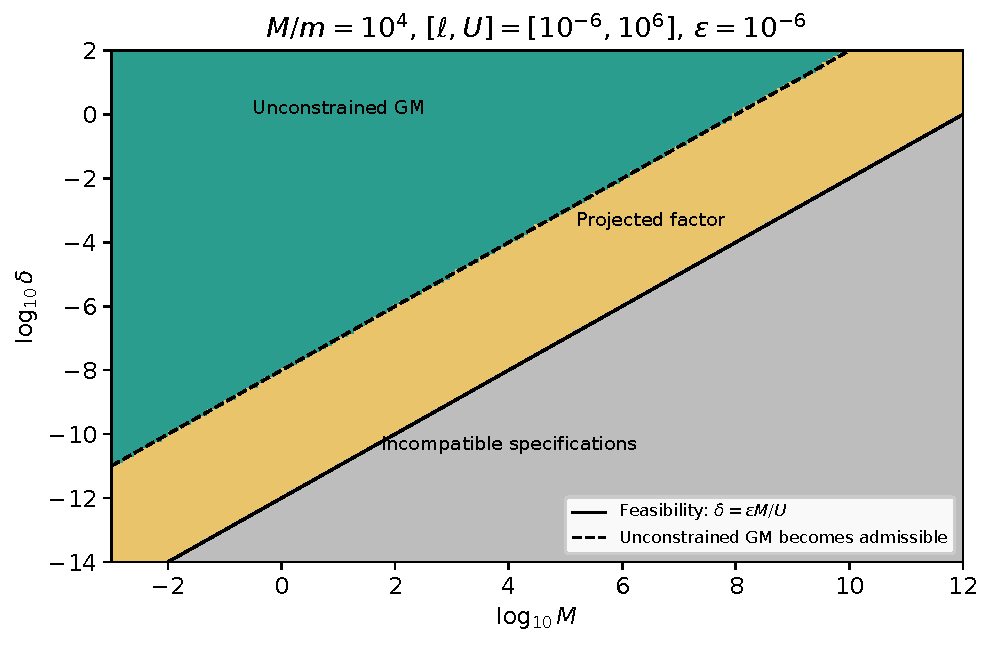
\includegraphics[width=.8\linewidth]{figs/research/budget-compatibility.pdf}
\caption{Exact compatibility regions for a row with fixed within-row spread. Below the
solid line, the residual budget conflicts with the coefficient ceiling. In the middle
region the constrained minimax factor is projected onto the admissible interval; above
the dashed line ordinary GM already satisfies it. This diagram concerns the conditional
row contract, before reserving any integer-rounding allowance}\label{fig:budget-compatibility}
\end{figure}

\section{Historical single-instance budget sensitivity}
The historical caso46e illustration uses budgets declared by a modeller, not measured
from an operating tolerance, so the natural objection is that admissibility was read off a
convenient choice. Table~\ref{tab:application-budget-sensitivity} scales all six declared budgets by a common multiplier and reports,
per constraint group, the tightest multiplier at which each kernel is still admissible on every
row of the group. Admissibility is monotone in the budget --- a larger $\delta$ only widens the
interval of Proposition~5.1 --- so the tightest multiplier with full coverage is the point at
which the contract starts to bind, and the data confirm the monotonicity on every group and
kernel.

All three kernels remain admissible on all 4,320 rows down to a multiplier of $10^{-4}$: the
declared budgets could be tightened ten thousandfold before any of them loses a row. The two
kernels the main text compares, the unit factor of Base and the geometric mean of Flat-GM,
survive to $10^{-5}$. Below that the groups separate in the way the proposition predicts: the
water balances, whose coefficients span the widest range, keep admitting the unit factor down to
$10^{-9}$, while the Euclidean kernel of Flat-L2 is the first to leave the admissible interval
on the four groups written in megawatts. The conclusion of the main text is therefore not an
artifact of the particular numbers declared; it would take a tolerance four orders of magnitude
tighter than a tenth of a megawatt to make the choice of kernel a question of admissibility
rather than of conditioning.

\begin{table}[tb]
\centering\small
\caption{Tightening the declared budgets of the application table. For each constraint group of
caso46e, the smallest common multiplier of the declared budgets at which the kernel is still
admissible on every row of the group, with $\epsilon=10^{-6}$ and the coefficient window
$[10^{-9},10^{9}]$. A multiplier of one is the budget declared in the main text; smaller means a
tighter tolerance. The sweep covers $10^{-16}$ to $10^{2}$.}
\label{tab:application-budget-sensitivity}
\begin{tabular}{lrrrr}
\toprule
Constraint group & Rows & \multicolumn{3}{c}{Tightest admissible multiplier} \\
\cmidrule(lr){3-5}
 &  & Base & Flat-GM & Flat-L2 \\
\midrule
Generation identities, demand cap & 1,080 & $10^{-5}$ & $10^{-5}$ & $10^{-4}$ \\
Generation definition, Bonete/Palmar & 720 & $10^{-5}$ & $10^{-5}$ & $10^{-4}$ \\
Production envelope tangents & 1,080 & $10^{-5}$ & $10^{-5}$ & $10^{-4}$ \\
Water balance, Bonete/Palmar & 720 & $10^{-9}$ & $10^{-7}$ & $10^{-5}$ \\
Water balance, Baygorria & 360 & $10^{-9}$ & $10^{-5}$ & $10^{-5}$ \\
Generation definition, Baygorria & 360 & $10^{-12}$ & $10^{-9}$ & $10^{-4}$ \\
\midrule
All groups & 4,320 & $10^{-5}$ & $10^{-5}$ & $10^{-4}$ \\
\bottomrule
\end{tabular}

\end{table}

The analysis is reproducible without an optimizer. The exported LP it reads is stored beside the
results, \path{results-revision/research-audit/application-budgets/caso46e-dummylp.lp.gz}, and
\texttt{make research-application-export} re-exports it from the instance with the solver-free
build and compares the two byte by byte; \texttt{make research-application-budgets} regenerates
both tables from it. That export is written by the repository's own serializer rather than by
Gurobi, as the archived one was: the two differ in the last digits of their decimal output, which
moves the reported quantities of one group by a relative $10^{-15}$ and nothing in either table.

\section{Additional OMS dispatch validation}
The additional protocol is frozen in
\path{results-revision/research-audit/oms-close-20261013/design.json}.
It uses the same 30 operational inputs, Gurobi 13.0.2, four threads, seed 42,
120 seconds and a 1\% gap. The separate pilot does not enter the results.
The six-model stage ablation selects positions 1, 8 and 15 in each archived class list.
All 132 exports retain objective, bounds and domains and are checked by named
row proportionality; the partial-stage factors have disjoint supports and multiply
to the full Role-Hybrid factors. A mechanical LP-serializer correction, made before
the first new optimization call, is recorded in \texttt{protocol-amendments.json}.

Execution resumed after an interruption with identical hardware and settings. Four
observations whose incumbent archives were empty were repeated under the unchanged
protocol and replaced, with the superseded CSVs and recovery criterion preserved in
\texttt{artifact-recovery.json}. They are not extra observations in the paired sample.

Ruiz-R4 freezes column factors at one and performs four coefficient-only infinity-norm
half-steps. Its final cumulative factor passes the same identity band and coefficient
window as the other policies. The historical C++ Ruiz option is not used. All
compressed LPs, named reference bases, factors, solution vectors and logs are stored.
\texttt{comparison-summary.csv} and \texttt{ablation-summary.csv} retain the paired
sample size for each aggregate; \texttt{runs.csv} preserves unfinished runs and their
PAR10 penalties. The 120-second local experiment is never pooled with the historical
1,800-second operational campaign.

The three physical precision scenarios use 0.01, 0.1 and 1 MW for power, and 100,
1,000 and 10,000 cubic metres for water. They are declared study objectives, not
operator tolerances. Algebraic budgets are read from the named generation/storage
coefficient or the hourly-flow conversion. Every row-level proposed factor, interval
and applied factor is retained in \texttt{factor-contracts.csv.gz}; it includes the
partial-stage policies on their six-model subset. The exported-row hypothesis is
$10^{-6}$ with zero rounding allowance for the interval audit. Actual physical
residuals and pointwise coefficient/RHS export defects are computed separately by
exact rational arithmetic on binary64 generator data and saved incumbents.
\texttt{physical-verification.csv} records these results by physical family and counts
observed violations of the exported-row hypothesis. Whole-model row, bound and
integrality diagnostics remain floating-point; dispatch optimality is not independently
certified. \texttt{make research-oms-check} replays the preserved exports and points,
checks every interval with rational endpoints and recomputes the comparison aggregates,
without calling an optimizer. The main text reports the compact comparison, final-policy
ablation and application-level budget sensitivity.

\section{Cross-run certificate audit}
\label{sec:stored-run-audit}
This exploratory audit, referenced briefly in the article's discussion, compares
reported objectives and dual bounds with numerically screened points. It includes
an objective difference of 54.7\% in the example below, without exact dispatch
feasibility certification or causal attribution. The separate activation study in
Section~\ref{sec:activation-followup} supplies independently checked exact feasible
witnesses of the actual imported exports.

The audit uses two stored campaigns: the solver-robustness campaign,
which was prepared, partly run and then stopped by decision, and the two replications of the
operational reconstruction. Neither is a census and neither was designed to estimate how often a
solver contradicts itself, so the counts below describe what occurred in the runs that exist.

The comparison rests on the stored verification. Each run's returned point is re-evaluated
against the original unscaled model, so a point accepted on a scaled export is still checked
where it has to hold, and \texttt{verif\_solver\_obj\_original} is its objective there. A point
the campaign tolerance merely accepted can be slightly infeasible, and an infeasible point
bounds nothing, so both the article and Table~\ref{tab:certificate-audit-detail} use only the
\emph{strict} tier: witnesses whose relative activity residual, bound violation and integrality
violation against the original model are each at most $10^{-9}$. This is a numerical
screen, not exact feasibility certification or a bound on objective perturbation.
The stopped campaign contains 4,542 recorded runs: 76 reported bounds lie above a
strictly screened witness across 26 instances, and 25 of those runs across nine instances
also report completion beyond the requested gap. In the 480-run operational replication,
the corresponding counts are 20 across six instances and nine across four. Base accounts
for five of the 25 completion discrepancies in the stopped campaign and one of nine in
the replication. These are counts of stored diagnostic discrepancies, not population rates
or independently certified invalid solver bounds.
The looser tier changes one
run and one instance, in the weaker of the two levels of the stopped campaign (77 runs across 27
instances instead of 76 across 26) and nothing at all elsewhere; the stored CSVs carry both
tiers in their own columns.

\begin{table}[htb]
\centering\small
\caption{Cross-run certificate audit by level and policy. ``Dual bound'' counts runs whose
reported bound lies above a numerically screened point of the same model; ``Certificate'' counts the subset
that also reported completion further from that point than the requested gap. Runs and
instances are the totals of that level.}
\label{tab:certificate-audit-detail}
\begin{tabular}{llrrrrrr}
\toprule
Campaign & Level & Runs & Inst. & Base & Flat-GM & Flat-L2 & Role-Hybrid \\
\midrule
Stopped campaign & Dual bound & 77 & 27 & 6 & 28 & 13 & 30 \\
 & Certificate & 25 & 9 & 5 & 9 & 1 & 10 \\
Operational replication & Dual bound & 20 & 6 & 1 & 6 & 3 & 10 \\
 & Certificate & 9 & 4 & 1 & 3 & 1 & 4 \\
\bottomrule
\end{tabular}

\end{table}

\paragraph{The extreme case.} On \path{v1_simple_000293}, one of the recombined Simple models,
eight runs exist at a 1\% gap and seed 1: four policies under each of Gurobi 13.0.1 and CPLEX
22.1.2, all recorded against the same \texttt{instance\_sha256}. Seven of them return an
objective between $-2.893\times10^8$ and $-2.913\times10^8$. The eighth, Gurobi on the unscaled
Base export, returns $-1.317\times10^8$ with status optimal, a reported gap of zero and a dual
bound equal to its objective. Its stored record shows one node explored against a root gap of
$1.22$, a wall time of 6~s, and three solver warnings: large bounds, large matrix coefficients
and large right-hand sides. Its returned point also passes the original-model numerical
screen, with relative activity violation $3.2\times10^{-14}$; the discrepancy concerns
objectives and bounds, without certifying exact feasibility or localizing a cause.
The strict witness of this instance is Gurobi on the Flat-GM export at $-2.909\times10^8$, with
relative activity residual $1.1\times10^{-13}$ and no bound or integrality violation; the
reported objective exceeds it by $1.592\times10^8$, which is $54.7\%$ of the magnitude of the
witness. A looser witness, Gurobi on Flat-L2 at $-2.913\times10^8$, does not meet the strict
residual threshold and is not used. CPLEX on the same unscaled file explored 6,151 nodes,
emitted no warnings and reached $-2.904\times10^8$.

The identical instance hashes support comparison of the stored outcomes. The discrepant
completion occurs on the unscaled export too, so the audit cannot attribute it uniquely to
external scaling. Neither exact dispatch optimality nor a cause inside the solver is
established by these records. The warnings motivate further numerical diagnosis; they do
not prove a particular failure mechanism.

\section{Independent verification and arithmetic checks}
The independent script \path{scripts/research/verify_saved_experiment.py} imports
neither the experiment runner nor an optimizer. For each of the 96 stored models it
enumerates all 4,096 binary assignments using integer activities, checks the reported
optimum, and then recomputes the acceptance decision from the saved point. It checks
the HiGHS/Gurobi archive with 3,456 distinct configuration keys, 288 abstentions and
768 dyadic exports. Running the same script with \texttt{-{}-root} set to
\path{results-revision/research-audit/budget-final-cplex} checks the CPLEX arm:
1,728 keys, 144 abstentions and 384 dyadic exports. Thus the two invocations cover
all three solvers: 5,184 planned configurations, 432 abstentions and 4,752 actual
optimizer calls, with 1,152 exact dyadic export checks. Both use the same 96 models,
whose CPLEX copies are byte-identical. \path{scripts/research/verify_stress_coverage.py}
reconciles the per-root verification records; \texttt{make research-check-python}
runs both invocations. Factor admissibility and dyadic multiplication are checked
rationally. The separate \texttt{research-claims} audit also enumerates and checks
the saved acceptance decisions for CPLEX.

A verified optimum requires an exactly feasible rounded binary point attaining the
enumerated objective, a returned point within $10^{-9}$ of that rounded point,
and bounds respected within $10^{-9}$. Raw-point residual budgets and integrality
errors are separate diagnostics. In particular, the verified-optimum label concerns
the rounded assignment; it does not claim exact feasibility of the raw floating-point
point. A failure of this conservative check does not by itself identify a solver bug.

Rational checks interpret each stored binary64 datum exactly. They do not recover
unrecorded real-valued physical data. Arbitrary-factor multiplication may change the
represented row by rounding even when its factor lies in the exact admissible
interval. The dyadic routine avoids this by intersecting the coefficient/budget
interval with exact exponent restrictions on every coefficient and the RHS.
It compares candidate centering objectives as rational numbers, because floating
logarithms can misclassify a near-midpoint as a tie.

Tests compare continuous interval projection with an independent linear program in
log coordinates, check positive re-emission, incompatible specifications, subnormal
and overflow boundaries, and a cancellation example where a floating-point residual
misses an exact unit violation. A native C++ integration test exercises the actual
LP writer with very small coefficients, RHS, bounds and objective values. The
serializer uses \texttt{max\_digits10} and general decimal notation so binary64
values survive decimal round-trip parsing. Serialization correctness and exact
multiplication are separate conditions; solver-internal transformations remain
outside both guarantees.

\section{Activation contracts and exact feasible witnesses}
\label{sec:activation-followup}
This exploratory extension uses the six archived SG-Ter-Mer inputs without the
documented total/local-demand inversion: instance001, instance005, instance022,
instance027, instance031 and instance046. It does not repair or replace inputs.
The existing numerical precision levels are applied explicitly to reservoir-volume
activation thresholds. They are study objectives, not operator tolerances or
measurements of error in the nonlinear plant model.

The coefficient-only L2 control projects its row factor onto $[10^{-9},10^9]$,
scales the whole row and RHS, and uses no identity band. This is a separate control,
not a renaming of the historical Flat-L2 policy. Budget-L2 uses the same kernel
and adds the admissible residual interval. On a volume activation
$M\varphi-v\le M-V$, the integer reserve is $E=M\gamma$. Default
$\gamma=10^{-5}$ exhausts the three volume budgets in this example. The guided
allowance is the largest power of two not exceeding
$\delta_V/(2\max_r M_r)$, capped at $10^{-5}$ and checked against Gurobi's
supported minimum. At demanding precision it is $2^{-28}$ in all six models.

For activation rows with finite boxes $|x_j|\le X_j$, we also reserve
\[
 \zeta_r=2^{-52}\left(\sum_j|a_{rj}|X_j+|b_r|\right).
\]
Normal binary64 products and round-trip decimal serialization give a conservative
forward-error allowance independent of the positive row factor. The selector
uses $\delta_r-E_r-\zeta_r$; rational checks subsequently verify the actual exported
defect against that allowance. Normality, coefficient limits and every factor
interval are checked. The resulting demanding projection changes exactly the
1,440 activation rows in each model and no other L2 factor. On instance046,
$\alpha$ increases from $10^{-9}$ to approximately $1.87\times10^{-8}$.
The allowance does not assert that a solver enforces its nominal tolerance:
observed exported and original residuals remain separate checks.

\paragraph{A rounding decision in original units.}
In the stored Base point of instance046, hour 18 has
$\varphi=0.9999996126403118$, $v=2066844230.148119$\,m\textsuperscript{3}
and a credited-power component $\theta=13.60595418958399$\,MW.
The activation is $12494793414.450399\,\varphi-v\le10427944344.323$;
the associated power bound is $\theta\le25.759667882689403\,\varphi$.
For the stored binary64 data, fixing $\varphi=1$ with continuous quantities
unchanged violates the activation by exactly $2537543057/524288$\,m\textsuperscript{3}.
Fixing it to zero instead violates the power bound by 13.606\,MW.
Thus neither binary choice meets the demanding or reference pair of study
budgets at that fixed continuous point. This certifies a need to change continuous
quantities or reject that rounded interpretation, not infeasibility of the MILP.

\paragraph{Comparison protocol and endpoints.}
The principal comparison has 72 assignments: six models, three seeds (1, 7, 42)
and four policies. Gurobi 13.0.2 uses four threads, 120 s, relative gap 1\%,
automatic internal scaling and presolve. L2-matched-int and Budget-L2 share
$\gamma=2^{-28}$ and primal tolerance $10^{-6}$; GM uses default integer
tolerance $10^{-5}$. L2-global-tight sets both tolerances to $10^{-9}$.
An eight-call, 60-second pilot on seed 17 is excluded. Additional controls on
instance046 use the same three principal seeds (27 assignments). A subsequent
presolve-off comparison fixes new seeds 11, 23 and 47 before its nine calls.
Preset reference/permissive sensitivity adds six calls. There are 114 nonpilot
calls, all retained, with their native logs, parameters and incumbent vectors.
Calls are sequential and these timings are not pooled with earlier campaigns.

\begin{table}[tb]
\centering\small
\caption{Activation follow-up on six models and three seeds. All 18 calls per
policy report completion. The Budgets column counts integer-rounded points passing
exact original-unit checks on all audited physical rows and activations. $B>U$ counts
reported bounds above an exact feasible objective of the same imported export,
allowing the larger of $10^{-6}$ objective units and eight bound ulps for display
rounding. Gap flags count cases satisfying $U<C-0.01|C|$, incompatible with the requested
completion criterion. Neither an unflagged bound nor budget compliance certifies
global optimality. Work is the geometric mean over all assigned calls, including
flagged completions; it must be interpreted with those flags.}
\label{tab:activation-bank}
\begin{tabular}{lrrrrr}
\toprule
Policy & Calls & Budgets & $B>U$ & Gap flags & Work\\
\midrule
GM & 18 & 18 & 3 & 0 & 1.397\\
L2, matched $\gamma$ & 18 & 18 & 7 & 6 & 0.958\\
Budget-L2 & 18 & 18 & 1 & 0 & 1.045\\
L2, global tight & 18 & 18 & 6 & 5 & 1.103\\
\bottomrule
\end{tabular}

\end{table}

\paragraph{Exact witness construction.}
Observed exactly integral states are fixed, substituted into the rows, and the
remaining LP is solved with SoPlex 8.1.0 and GMP 6.2.1 in rational mode.
Its coefficients are full plain decimal expansions of the original binary64
numbers, not newly rounded decimal data. A separate Python \texttt{Fraction}
checker verifies all 10,080 original rows, all 6,120 variable bounds and all
1,440 integer domains, and recomputes the exact objective. Twenty witnesses
cover the native GM, L2-window and Budget-L2 exports in the six models,
Base on instance046, and its reference-budget export. They are feasible
points supplying upper bounds, not global optima. Each comparison identifies
the actual imported model by SHA-256. The Base witness also applies to both
dyadic controls after verifying exact proportionality of every coefficient
and RHS. This prevents export-rounding differences from serving as an
unsupported equivalence assumption. Tight-M/indicator controls have primal
checks but no separate native-export witness in the bound comparison.

\begin{table}[tb]
\centering\small
\caption{Controls on instance046, with columns defined in
Table~\ref{tab:activation-bank}. Upper panel: seeds 1, 7 and 42; presolve is
automatic except where stated. Lower panel: fresh seeds 11, 23 and 47 with
presolve disabled throughout. A dash indicates that no native-export witness
was supplied for that reformulation, not that its bounds were certified.
The dyadic L2 control still has one contradicted completion despite exact
row proportionality. NumericFocus 3 is an effective existing alternative.}
\label{tab:activation-controls}
\begin{tabular}{lrrrrr}
\toprule
Policy & Calls & Budgets & $B>U$ & Gap flags & Work\\
\midrule
Base & 3 & 0 & 0 & 0 & 51.646\\
Ruiz-R4 & 3 & 1 & -- & -- & 50.305\\
L2, presolve off & 3 & 0 & 3 & 3 & 0.578\\
L2, NumericFocus 3 & 3 & 3 & 0 & 0 & 26.629\\
L2, dyadic & 3 & 3 & 1 & 1 & 8.887\\
Budget-L2, dyadic & 3 & 3 & 0 & 0 & 13.479\\
GM, IntegralityFocus & 3 & 3 & 3 & 0 & 13.801\\
GM, tight $M$ & 3 & 2 & -- & -- & 12.594\\
GM, indicators & 3 & 3 & -- & -- & 14.724\\
\bottomrule
\end{tabular}

\par\medskip
\begin{tabular}{lrrrrr}
\toprule
Policy & Calls & Budgets & $B>U$ & Gap flags & Work\\
\midrule
L2, matched $\gamma$ & 3 & 0 & 3 & 3 & 0.597\\
Budget-L2 & 3 & 3 & 2 & 0 & 4.485\\
L2, global tight & 3 & 3 & 3 & 3 & 0.577\\
\bottomrule
\end{tabular}

\end{table}

In the fresh-seed comparison, L2 gives a 4,837.338\,m\textsuperscript{3}
activation residual in all three calls. Budget-L2 reduces the maximum to
$1.4782\times10^{-5}$\,m\textsuperscript{3}. Global tightening reduces it to
zero but retains the cost near $-572330$ and zero reported gap, contradicted
by an exact feasible cost near $-799086$. The geometric mean optimizer work is
0.597 for L2, 4.485 for Budget-L2 and 0.577 for global tightening. The fast
controls therefore cannot be regarded as equivalent successful computations.

\begin{table}[tb]
\centering\small
\caption{Preset numerical volume targets on instance046 with seeds 1, 7 and 42.
Changed rows counts differences from the coefficient-window L2 export.
The demanding row is the corresponding subset of the principal comparison.
All nine points meet their primal budgets, while the looser specifications
permit contradicted completion claims. This is sensitivity of one
configuration, not an estimated failure rate.}
\label{tab:activation-sensitivity}
\begin{tabular}{lrrrrr}
\toprule
Scenario & $\delta_V$ (m$^3$) & $\gamma$ & Changed rows & Budgets & Gap flags\\
\midrule
Demanding & 100 & $2^{-28}$ & 1,440 & 3/3 & 0/3\\
Reference & 1,000 & $2^{-25}$ & 1,440 & 3/3 & 1/3\\
Permissive & 10,000 & $2^{-22}$ & 0 & 3/3 & 3/3\\
\bottomrule
\end{tabular}

\end{table}

Selection and round-trip export are measured separately in three fixed-order
paired repeats per model, including budget-specific unit lookup and reserves
but excluding common LP reading. Every timed export is byte-identical to its
frozen counterpart. Median times are 0.354--0.360 s for L2-window and
0.497--0.505 s for Budget-L2, an additional approximately 0.14 s.
The solver-call times include import and optimization, exclude these preparation
measurements and verification, and are preserved separately. All data and
solver-free replay programs are under
\path{exploration/oms-followup-20261014}. The observed benefits concern the
chosen target, generator, solver and settings; the reference sensitivity and
remaining bound discrepancies explicitly exclude an optimality guarantee.

\FloatBarrier
\section{Sensitivity to incumbent initialization}
\label{sec:si-incumbent}
\begingroup
\widowpenalty=10000
\clubpenalty=10000
\paragraph{Diagnostic question and protocol.}
This auxiliary experiment tests whether the observed completion advantage of external
scaling persists when both representations receive the same incumbent. Three known
SG-Ter-Mer models are selected retrospectively: instance001 and instance003 previously
favored GM, while instance042 favored Base. They are not an independent validation
sample. Each retains 6,120 variables, 10,080 rows and 1,440 binaries. The bank uses native
MPS inputs and frozen power-of-two GM factors, rather than the historical LP exporter and
arbitrary-factor policies; it does not retrospectively identify the cause of that campaign.
Base and GM change only complete rows and their RHS, with exact proportionality checked.
The GM policy uses the coefficient window $[10^{-9},10^9]$ and an identity band
$[0.5,2]$ on proposals, followed by projection onto the admissible power-of-two grid.

Base/GM, without a supplied incumbent (Cold) or with a common MIP start (CommonStart),
and three new seeds (503, 509, 521) give 36 sequential MILP calls. Gurobi 13.0.2 uses
four threads, limits of 12 seconds and 12 work units, relative gap $10^{-3}$, primal
tolerance $10^{-6}$, integer tolerance $10^{-5}$, IntegralityFocus=0, and automatic
presolve and internal scaling. The schedule and source/input hashes are fixed before
the calls. All assignments, limits, native logs, candidates and endpoints are retained.

\paragraph{Common reference and its cost.}
For each case, only the integer pattern of the archived GM run at seed 307 is used.
A single SoPlex 8.1.0/GMP continuation, limited to 15 seconds, produces an exactly
feasible point and matching primal/dual values for that fixed-pattern LP. These are
not global MILP optima. The same binary64 conversion of the rational point is supplied
to Base and GM; original-row, exported-row, bound and integer checks are retained
separately. All 18 starts are loaded, and their integer pattern and objective are
observed at node zero and zero recorded work. Acceptance is checked rather than assumed.

The three new reference acquisitions, including LP export and checking, take
1.79--1.84 seconds each. Their patterns were obtained by earlier GM runs requiring
approximately 8.186, 4.931 and 0.451 native work units for 001, 003 and 042 respectively.
The reference is therefore offline diagnostic information, not a free input to a
proposed solution algorithm. Acquisition, construction and checking costs are separate
from the optimizer-work comparison in Table~\ref{tab:incumbent-initialization}.

\begin{table}[tb]
\centering\small
\caption{Auxiliary common-incumbent diagnostic on three known cases and seeds 503,
509 and 521. Completion counts calls reaching the requested native gap, not certified
global optimality. Work is the median over all three assigned calls, including censored
ones; ratios involving those censored calls are not speedups. Both zero work values on
warm instance042 are native reports, not zero total cost, and are not divided into ratios.}
\label{tab:incumbent-initialization}
\begin{tabular}{llrrrr}
\toprule
Case & Initialization & Base completes & Base work & GM completes & GM work \\
\midrule
001 & Cold & 0/3 & 12.0001 & 3/3 & 5.4909 \\
001 & CommonStart & 3/3 & 6.4158 & 3/3 & 6.7719 \\
003 & Cold & 0/3 & 12.0002 & 3/3 & 4.3099 \\
003 & CommonStart & 3/3 & 4.7903 & 3/3 & 4.6932 \\
042 & Cold & 3/3 & 0.3284 & 3/3 & 0.4928 \\
042 & CommonStart & 3/3 & 0.0000 & 3/3 & 0.0000 \\
\bottomrule
\end{tabular}

\end{table}

With the common start, the paired GM/Base work ratios are 1.0555, 1.0519 and 1.3686
on 001, and 0.9957, 1.1114 and 0.7683 on 003. Thus the cold-start completion advantage
disappears in both cases; GM has higher work in all three warm 001 pairs and mixed
differences on 003. Where a root relaxation is logged, objectives coincide at printed
precision in all 15 Base/GM pairs. This is neither exact LP certification nor an
independent contribution: positive row scaling preserves the mathematical LP in exact
arithmetic. Some root objectives change between Cold and CommonStart, and no root LP
is logged for warm 042. A start can affect objective cutoffs, presolve and later search;
the intervention does not isolate one heuristic or prove a unique cause of the effect.

\paragraph{Independent checks and reproducibility.}
All 15 unique final integer patterns enter a queue fixed before the posthoc exact-LP
checks, with a five-second limit and no replacements. Thirteen have matching exact
primal/dual optima; two remain unknown, both from Base-Cold 001, which did not reach
the requested gap. The common-start comparisons have certified continuations at
comparable costs. Conditional pattern optima are not global MILP lower bounds.
No reported bound exceeds the common exact feasible objective in this experiment;
absence of contradiction does not validate global bounds.

The independent replay reconstructs references and fixed-pattern LPs from original
binary64 rows, verifies their rational primals and duals, checks row proportionality,
recomputes candidate objectives and final-point residuals after integer rounding,
and verifies start acceptance and all final-pattern assignments. Four endpoint tests
passed before the MILP calls. Data, protocols, sources, native records, exact certificates
and the two unknown outcomes are supplied under
\path{exploration/oms-root-attribution-20261015/}. This selected-case diagnostic
qualifies mechanism attribution; it provides neither a general scaling ranking nor
a new incumbent-generation algorithm.

\FloatBarrier
\endgroup
\section{Matched IntegralityFocus control and complete workflow cost}
\label{sec:si-if1-workflow}
Twelve principal calls repeat instance046: L2-matched-int/Budget-L2,
IntegralityFocus=0/1 and seeds 11, 23, 47. Each fresh process constructs the original
C++ model once and runs selection, export, import, solve and verification. Exports
match their historical SHA-256 values. Gurobi 13.0.2 uses four threads, 120 seconds,
1\% gap, primal/integer tolerances $10^{-6}$/$2^{-28}$, presolve off, automatic
internal scaling and no MIP start. Budgets, reserves and factors are unchanged.

IF1 and IF0 produce identical saved points, objectives, bounds and work in all six
matched pairs. All returned integer coordinates are exactly integral. L2 retains
the 4,837.338\,m\textsuperscript{3} activation violation; Budget-L2 limits it to
$1.4782\times10^{-5}$\,m\textsuperscript{3}, while two of its three reported bounds
still exceed exact feasible objectives. Thus IF1 does not repair this configuration;
the result makes no claim about its general effectiveness or MILP optimality.

The three Budget-L2 Work values, unchanged from the earlier presolve-off campaign,
are 3.6054776613, 4.9754950464 and 5.0281587478 for seeds 11, 23 and 47.
Their geometric mean is 4.4847271866 (4.485 in Table~S12 and historical main-text Table~11 of v1.3.8);
their median is 4.9754950464 (4.975 here and in the workflow note). The different
summaries, rather than a configuration change, explain the apparent discrepancy.

\begin{table}[tb]
\centering\small\setlength{\tabcolsep}{4pt}
\caption{Matched IF control and full prototype costs. Upper: budget and bound/gap
definitions follow Table~S11; Work is the median. Lower: median wall seconds.
Generate includes C++ launch, input, construction and Base writing; Select/export
covers factors and scaled writing; Import/check covers native setup and model equality.
Total includes the entire fresh process, also startup, reading, metadata, integrity,
extraction and persistence. Stages shown are not exhaustive; medians need not add.
Shared-machine timings describe this prototype and do not establish general performance.}
\label{tab:if1-workflow}
\begin{tabular}{lrrrrrr}
\toprule
Policy & Calls & Budgets & Max. $v_V$ (m$^3$) & $B>U$ & Gap flags & Work\\
\midrule
L2-window, IF0 & 3 & 0/3 & 4,837.338 & 3 & 3 & 0.597\\
L2-window, IF1 & 3 & 0/3 & 4,837.338 & 3 & 3 & 0.597\\
Budget-L2, IF0 & 3 & 3/3 & $1.478\times10^{-5}$ & 2 & 0 & 4.975\\
Budget-L2, IF1 & 3 & 3/3 & $1.478\times10^{-5}$ & 2 & 0 & 4.975\\
\bottomrule
\end{tabular}

\par\medskip
\begin{tabular}{lrrrrrr}
\toprule
Policy & Generate & Select/export & Import/check & Solve & Verify & Total\\
\midrule
L2-window, IF0 & 0.115 & 0.428 & 0.114 & 0.639 & 0.269 & 2.070\\
L2-window, IF1 & 0.115 & 0.367 & 0.099 & 0.533 & 0.228 & 1.768\\
Budget-L2, IF0 & 0.065 & 0.514 & 0.097 & 4.788 & 0.237 & 6.231\\
Budget-L2, IF1 & 0.064 & 0.528 & 0.099 & 4.955 & 0.239 & 6.380\\
\bottomrule
\end{tabular}

\end{table}

The first twelve-call pass repeatedly copied binding vectors in
the import checker. Caching them once and repeating all treatments leaves every
point and native endpoint unchanged. These 24 calls are not pooled as independent
samples; principal timings use the second pass. Compilation and prior witness
acquisition are offline costs; revalidating both exact witnesses is timed separately.
The independent replay checks 103,680 physical row/point combinations before/after
rounding and the same-model bound/gap refutations. Sources, all stages, both passes,
the two existing witnesses and four endpoint tests are supplied under
\path{exploration/oms-if1-workflow-20261015/}.

\FloatBarrier
\section{Fully matched accuracy and numerical-remedy comparison}
\label{sec:si-matched-accuracy}
A fixed factorial comparison uses the same six demand-inversion-free models as
Section~\ref{sec:activation-followup}, seeds 11, 23, 47, automatic/off presolve,
and L2, Budget-L2, L2-tight and L2-NF3. The 144 terminal comparisons use Gurobi
13.0.2, four threads, 120 seconds, 1\% gap, ScaleFlag=$-1$,
IntegralityFocus=0 and no MIP start. L2 and Budget-L2 share primal/integer
tolerances $10^{-6}$/$2^{-28}$; L2-tight uses $10^{-9}$ for both; L2-NF3 adds
NumericFocus=3 to the matched L2 settings. Each fresh process constructs the C++
model once. Base and scaled exports reproduce their archived hashes exactly;
only the 1,440 activation factors differ between L2 and Budget-L2 in each model.
The original-unit targets, conversion, integer and export reserves are unchanged.

The randomized order and endpoints were fixed before optimization. A host reboot
interrupted the 38th attempt; its partial files are preserved, the preceding
37 complete calls are retained, and only the interrupted assignment is repeated
before continuing the original order. Thus 145 native attempts produce 144 terminal
comparisons, with one separately recorded external failure of delivery. There are
no new reference LP solves. The reader-only replay rechecks twelve supplied exact
feasible witnesses and all saved candidates using rational binary64 arithmetic.

All policies meet the primal budgets under automatic presolve. With presolve off,
only L2 on instance046 fails them, in all three seeds. Budget-L2 and both numerical
remedies meet every primal budget. Budget-L2 retains one/three bound discrepancies
under automatic/off presolve, whereas NumericFocus=3 has none detected in either
panel. Their paired geometric-mean Work ratios, Budget-L2/NumericFocus=3, are
0.361 and 0.227 respectively over all 18 pairs per panel. These compare terminal
primal delivery, not equally certified optimization outcomes; absence of a known
contradiction is not a bound certificate. The fully matched controls clarify the
cost and remaining limitation without extending primal recovery to a second model.

\begin{table}[tb]
\centering\small\setlength{\tabcolsep}{3pt}
\caption{Fully matched numerical remedies. Upper: each policy has 18 terminal calls
per presolve setting; ``Budgets'' counts points meeting all 4,320 audited rows after
integer rounding. Max. $v_V$ is the largest activation violation in
m\textsuperscript{3}; $B>U$ and Gap flags follow Table~S11. Limits counts native
time limits. Work is the geometric mean of all terminal calls, including flagged
completions; Total is the median entire fresh-process time in seconds. Lower:
per-model compliance among three seeds with presolve disabled. Absence of a bound
or gap flag does not certify optimality. The interrupted attempt is retained
separately rather than imputed or counted as a completed replicate.}
\label{tab:matched-accuracy}
\resizebox{\linewidth}{!}{\begin{tabular}{llrrrrrrr}
\toprule
Presolve & Policy & Budgets & Max. $v_V$ & $B>U$ & Gap flags & Limits & Work & Total\\
\midrule
Auto & L2 & 18/18 & 4.768e-07 & 5 & 3 & 0 & 1.59 & 1.944\\
Auto & Budget-L2 & 18/18 & 0.0001123 & 1 & 0 & 0 & 1.106 & 2.17\\
Auto & L2-tight & 18/18 & 0 & 5 & 3 & 0 & 1.516 & 1.894\\
Auto & L2-NF3 & 18/18 & 0 & 0 & 0 & 0 & 3.063 & 2.295\\
Off & L2 & 15/18 & 4837 & 8 & 8 & 0 & 0.2904 & 1.343\\
Off & Budget-L2 & 18/18 & 1.478e-05 & 3 & 0 & 0 & 0.6023 & 1.795\\
Off & L2-tight & 18/18 & 2.384e-07 & 8 & 8 & 0 & 0.2888 & 1.369\\
Off & L2-NF3 & 18/18 & 0 & 0 & 0 & 0 & 2.648 & 2.22\\
\bottomrule
\end{tabular}
}
\par\medskip
\begin{tabular}{lrrrr}
\toprule
Instance & L2 & Budget-L2 & L2-tight & L2-NF3\\
\midrule
instance001 & 3/3 & 3/3 & 3/3 & 3/3\\
instance005 & 3/3 & 3/3 & 3/3 & 3/3\\
instance022 & 3/3 & 3/3 & 3/3 & 3/3\\
instance027 & 3/3 & 3/3 & 3/3 & 3/3\\
instance031 & 3/3 & 3/3 & 3/3 & 3/3\\
instance046 & 0/3 & 3/3 & 3/3 & 3/3\\
\bottomrule
\end{tabular}

\end{table}

Complete process times include startup, C++ generation/Base writing, metadata,
factor selection, scaled export, native import/equality checks, optimization,
extraction, verification and persistence. Disjoint stages and objectives are
retained for every call. Compilation and prior witness acquisition are offline;
current witness revalidation is timed separately. Wall times span a reboot and
changing shared-machine load, so native Work is the primary effort measure.
The endpoint is terminal budget delivery at the native stopping rule, not time
to the first verified incumbent or a precision--cost frontier over multiple budgets.
Known models and previously used seeds provide within-family confirmation,
not external validation. Sources, every outcome, the interrupted attempt and
paired cost summaries are supplied under
\path{exploration/oms-matched-accuracy-20261016/}.

\FloatBarrier
\section{Multi-budget precision--effort sensitivity}
\label{sec:si-frontier}
The six known SG-Ter-Mer models are paired at seeds 59,71,89 under automatic/off
presolve, seven volume targets and a fixed 0.01 MW power target. The common
integer tolerance is $10^{-9}$, selected before optimization to study the full
budget range; it differs from $2^{-28}$ in Table~S16. Other settings match that
study, including 120 seconds, four threads and a 1\% requested gap. L2-tight uses
both tolerances $10^{-9}$; L2-NF3 adds NumericFocus=3 to the matched L2 control.
Of 360 randomized assignments, 30 abstain before solving because the uniform
integer-rounding reserve exhausts 10\,m\textsuperscript{3} in five models. The
sixth admits that budget. This is incompatibility of a sufficient contract, not
MILP infeasibility. All remaining 330 calls and 31 exact native-export feasible
witness acquisitions are retained. No fresh MILP run is needed for the replay.

The criterion fixed before solving requires at least four models to meet the
targets in all three seeds at two adjacent budgets, with lower paired geometric
work than NF3, no more detected bound contradictions and at most 1\% worsening
in candidate cost. All six qualify at 30 and 100\,m\textsuperscript{3} under
automatic presolve. Both policies pass every primal target and have zero detected
bound/gap contradictions there. Work ratios by model range from 0.128 to 0.668
at 30\,m\textsuperscript{3}, and 0.072 to 0.585 at 100\,m\textsuperscript{3}.
This is a descriptive comparison within known models, not external validation
or certification of their reported MILP bounds. Primal recovery over L2 still
occurs only on instance046 with presolve disabled.

\begin{table}[tb]
\centering\small\setlength{\tabcolsep}{3pt}
\caption{Prespecified sensitivity. Calls counts executed Budget-L2 calls out of
18 assignments; the missing 15 at 10\,m\textsuperscript{3} in each panel are
abstentions. Budgets counts successful rounded points. B/G denotes bound/gap
contradictions against exactly feasible witnesses of the same binary64 export.
NF3 has zero detected B/G flags and satisfies all targets in both panels.
Work and complete-time ratios are paired geometric means against NF3 on the
same executed cases/seeds. All controls are resolved once per case/seed/presolve
and checked at every target. At 3,000 and 10,000\,m\textsuperscript{3}, Budget
exports equal L2; these are not independent representations. Lower effort or
absence of a detected contradiction does not certify MILP optimality.}
\label{tab:precision-frontier}
\resizebox{\linewidth}{!}{\begin{tabular}{lrrrrrrr}
\toprule
Presolve & $\delta_V$ & Calls & Budgets & B/G & L2 B/G & $W/W_{\rm NF3}$ & $T/T_{\rm NF3}$\\
\midrule
Auto & 10 & 3/18 & 3/3 & 0/0 & 5/4 & 0.567 & 0.969\\
Auto & 30 & 18/18 & 18/18 & 0/0 & 5/4 & 0.411 & 0.704\\
Auto & 100 & 18/18 & 18/18 & 0/0 & 5/4 & 0.362 & 0.629\\
Auto & 300 & 18/18 & 18/18 & 1/0 & 5/4 & 0.364 & 0.688\\
Auto & 1000 & 18/18 & 18/18 & 6/6 & 5/4 & 0.496 & 0.874\\
Auto & 3000 & 18/18 & 18/18 & 5/4 & 5/4 & 0.487 & 0.811\\
Auto & 10000 & 18/18 & 18/18 & 5/4 & 5/4 & 0.487 & 0.854\\
Off & 10 & 3/18 & 3/3 & 0/0 & 9/9 & 0.599 & 0.943\\
Off & 30 & 18/18 & 18/18 & 1/0 & 9/9 & 0.226 & 0.579\\
Off & 100 & 18/18 & 18/18 & 3/2 & 9/9 & 0.188 & 0.561\\
Off & 300 & 18/18 & 18/18 & 6/6 & 9/9 & 0.119 & 0.499\\
Off & 1000 & 18/18 & 15/18 & 9/9 & 9/9 & 0.115 & 0.500\\
Off & 3000 & 18/18 & 15/18 & 9/9 & 9/9 & 0.114 & 0.479\\
Off & 10000 & 18/18 & 18/18 & 9/9 & 9/9 & 0.114 & 0.496\\
\bottomrule
\end{tabular}
}
\end{table}

Complete process time includes startup, generation once, metadata, selection,
export, import/equality checking, solving, extraction, original-row verification
and persistence. Compilation and witness acquisition are separate. On the shared
host, the aggregate time ratios at 30/100\,m\textsuperscript{3} are 0.704/0.629;
the 30\,m\textsuperscript{3} cycle is nevertheless slower in three inexpensive
models. No isolated hardware speedup is claimed. The 36 automatic-presolve
Budget points in this band satisfy the observed exported-row hypothesis:
no audited row exceeds $\epsilon=10^{-6}$ and the maximum is below $1.5\times10^{-10}$.
That observation is checked separately from factor admissibility and original-unit
residuals. With larger budgets or presolve off, Table~S17 retains adverse results.
Sources and all outcomes are in \path{exploration/oms-frontier-20261016/}.

\FloatBarrier
\section{Isolated native-selector integration}
An experimental hook applies the selector to the C++ generator's in-memory rows,
choosing all factors before modifying any row and exporting only once. The
original generator and its formulation are unchanged. Both arms use the same
isolated $-O2$ executable: Python disables the hook, exports Base, reconstructs
metadata and applies the reference selector; C++ enables the hook. Exact rational
intervals and reserves use Boost 1.74 multiprecision. At 0.01 MW/100\,m\textsuperscript{3}
and integer allowance $10^{-9}$, all factors, matrix/RHS values, objectives, bounds
and integer domains match the Python implementation on all six models, for L2
and Budget-L2. The independent replay checks 120,960 paired rows and 25,920 contracts.

\begin{table}[tb]
\centering\small
\caption{Two separate Budget-L2 implementation benchmarks. Preparation reports
medians of seven repeats per arm/model; speedup is Python/C++.
The complete cycle reports geometric means over seeds 59, 71, 89; its ratio is
C++/Python, with aggregate paired ratio 0.824. The former includes startup,
generation, selection, export and persistence; the latter additionally includes
native import/data checks, solving and physical verification. Compilation and
prior witness acquisition are separate. These are shared-host measurements,
not general hardware speedups.}
\label{tab:native-selection-cost}
\textbf{Standalone preparation}\par\smallskip
\begin{tabular}{lrrr}
\toprule
Model & Python (s) & C++ (s) & Preparation speedup\\
\midrule
001 & 1.318 & 0.265 & 4.97\\
005 & 1.167 & 0.315 & 3.70\\
022 & 1.167 & 0.315 & 3.71\\
027 & 1.368 & 0.215 & 6.37\\
031 & 1.318 & 0.315 & 4.18\\
046 & 1.168 & 0.315 & 3.70\\
\bottomrule
\end{tabular}

\par\medskip\textbf{Complete process}\par\smallskip
\begin{tabular}{lrrr}
\toprule
Model & Python (s) & C++ (s) & C++/Python time\\
\midrule
001 & 4.378 & 3.974 & 0.908\\
005 & 1.636 & 1.218 & 0.744\\
022 & 1.620 & 1.184 & 0.731\\
027 & 2.874 & 2.472 & 0.860\\
031 & 1.586 & 1.185 & 0.747\\
046 & 10.555 & 10.416 & 0.987\\
All 18 pairs & -- & -- & 0.824\\
\bottomrule
\end{tabular}

\end{table}

The corrected pass contains 168 timed preparations across both kernels, plus 24
preflight preparations. An earlier complete pass is retained: its C++ audit CSV
failed to quote row names containing commas. After correcting that format, the
entire identical design was repeated; every model export matches the first pass.
Thus 336 timed and 48 preflight preparations are supplied, with no optimizer call.
Part of standalone startup savings may overlap imports needed by a full solver
workflow, so the speedup is not applied to historical optimization times.
The prototype is under \path{exploration/oms-native-selector-20261016/}.

The subsequent complete-cycle benchmark fixes 36 calls in randomized paired
blocks on the same six models. Both arms read original-model metadata within
the measured process; Python disables the native selector and C++ enables it
in the same executable. All ordered binary64 model data, including row and
column order, match. All 18 pairs have identical points, native endpoints and
work. Paired time ratios by model range from 0.731 to 0.987, with aggregate
0.824; the 3.70--6.37 preparation speedups therefore are not extrapolated.
No other research solver campaign was run concurrently with this benchmark;
system load was recorded and all repetitions retained. Complete records and
independent checks are under
\path{exploration/oms-followup-20261017/native-cycle/}.

\FloatBarrier
\section{Exact global-LP reference intervals}
The six original Base models admit a supplementary verification independent of
their reported solver bounds. All 1,440 binary variables are relaxed, preserving
their $[0,1]$ bounds; no integer pattern is fixed in this LP. SoPlex 8.1.0 with
GMP obtains an exact primal/dual solution using the rational values of the original
binary64 coefficients, RHS, costs and bounds. The checker independently rebuilds
all inequalities, including variable bounds, verifies dual signs and $A^T\pi=c$,
and checks primal/dual objective equality. The dual therefore provides a genuine
global lower bound $L$ for the original MILP.

Separately, exactly feasible integer witnesses provide $U$. Their construction
uses a fixed-pattern LP, but only their verified primal vectors are used here;
that LP's dual is not a global MILP bound. Table~S19 reports the resulting
intervals. Negative objectives use width $(U-L)/|U|$. Equality is tested rationally,
not by comparing rounded displays. Three reference witnesses are certified within
1\%, and instance031 is certified exactly optimal. Wider intervals on the other
three models do not certify their reported 1\% gaps. These are original-Base
reference certificates, not a claim that a floating row export, a tolerance-feasible
native vector or every point in Tables~S16--S17 has a certified optimality gap.

\begin{table}[tb]
\centering\small\setlength{\tabcolsep}{3pt}
\caption{Verified original-model intervals from six unfixed exact LP relaxations
and six complete exact integer witnesses. Displayed costs are rounded; certificates
retain exact rationals. A width over 1\% is an unresolved interval, not evidence
that the integer optimum is known or that the relaxation gap equals that width.}
\label{tab:global-lp-certificates}
\resizebox{\linewidth}{!}{\begin{tabular}{lrrrl}
\toprule
Model & Global LP $L$ & Integer witness $U$ & Width (\%) & Verified conclusion\\
\midrule
001 & -1208494.856 & -989879.474 & 22.085 & Interval only\\
005 & -2558473.761 & -2540302.931 & 0.715 & Within 1\%\\
022 & -293986.477 & -292995.512 & 0.338 & Within 1\%\\
027 & -1615641.968 & -1598079.853 & 1.099 & Interval only\\
031 & -1542528.000 & -1542528.000 & 0.000 & Exact optimum\\
046 & -840709.945 & -799086.098 & 5.209 & Interval only\\
\bottomrule
\end{tabular}
}
\end{table}

The six global-LP construction/solve/check cycles cost 23.98 seconds in total on
the shared host; acquisition of the six integer witnesses is additional and
recorded separately. Replaying supplied primal/dual certificates requires no
optimizer. Sources and duals are under \path{exploration/oms-global-lp-20261016/};
the supplied \path{exploration/oms-joint-contracts-20261016/base-witnesses/} holds
the original-Base integer witnesses. The separate row/column research prototype
is outside the row-scaling claims of this manuscript.

\FloatBarrier
\section{Independent batch-scheduling transfer}
Eight prescribed horizons (8,10,12,16,20,24,32,40) use the archived
STN-Scheduler implementation of the Kondili batch-scheduling example, independent
of the hydrothermal generator. Horizons 10 and 12 are known anchors from an
earlier pilot that found no added primal benefit; the other six are new horizons
of the same external example, not six independent application families.
Source commit, license and complete model data are retained in the artifact.
Mass budgets are $10^{-5}$ kg (10 mg), logical budgets $10^{-5}$ and financial
budgets $10^{-3}$ source monetary units. These are numerical study goals,
not industrial accuracy standards.

All four controls use exact dyadic row/RHS export, the same coefficient window,
integer tolerance $10^{-9}$, automatic presolve, four threads, a 30-second limit
and a requested 1\% gap. Seeds 131,137,149 and all 96 assignments are fixed before
solving. L2-tight changes FeasibilityTol from $10^{-6}$ to $10^{-9}$; NF3 adds
NumericFocus=3. The integer tolerance is already $10^{-9}$ in every arm.
A pre-optimization construction check exposed the upstream dependence of
ConstraintList names/order on Python sets. The correction verifies the complete
mathematical row multiset, including duplicates, then restores the already frozen
row order. The failed preflight and source-only amendment are retained; no model,
export, assignment or optimizer result was changed.

\begin{table}[!htbp]
\centering\small
\caption{Independent batch-scheduling checks. Entries count returned points meeting
all original-row and variable-bound budgets after integer rounding. All integers
are retained. Changed rows compares exact dyadic Budget-L2 with matched dyadic L2.
The final row totals 24 calls per policy. Budget delivery is not exact feasibility
or a certificate of the reported MILP bound or gap. NF3's sole failing point has
111.041 mg capacity violation against 10 mg; the contractual bound is 8.2 mg.}
\label{tab:external-transfer}
\begin{tabular}{lrrrrr}
\toprule
Horizon & Changed rows & L2 & Budget-L2 & L2-tight & L2-NF3\\
\midrule
8 & 72 & 3/3 & 3/3 & 3/3 & 3/3\\
10 & 88 & 3/3 & 3/3 & 3/3 & 3/3\\
12 & 104 & 3/3 & 3/3 & 3/3 & 3/3\\
16 & 136 & 3/3 & 3/3 & 3/3 & 3/3\\
20 & 168 & 3/3 & 3/3 & 3/3 & 3/3\\
24 & 200 & 3/3 & 3/3 & 3/3 & 3/3\\
32 & 264 & 3/3 & 3/3 & 3/3 & 3/3\\
40 & 328 & 3/3 & 3/3 & 3/3 & 2/3\\
All & 1360 & 24/24 & 24/24 & 24/24 & 23/24\\
\bottomrule
\end{tabular}

\end{table}

Table~S20 verifies transfer of the procedure: Budget-L2, L2 and L2-tight each pass
24/24 checks, and NF3 passes 23/24. At horizon 40 and seed 149, the NF3 point has
$W=0$ and $B=1.110407442\times10^{-4}$ kg in the capacity row $B-200W\le0$.
Its violation is 111.041 mg against the 10 mg target, despite exact integer
coordinates. L2's factor $2^{-8}$ yields observed exported violation
$4.338\times10^{-7}<10^{-6}$. Budget-L2 selects $2^{-3}$: its conditional
rounded-original-row bound is $8+0.2=8.2$ mg, within the target. The checked
Budget-L2 point meets the target. Matched L2 also passes all checks; this example
does not establish a unique primal recovery over that control or general
computational superiority. Native solves are short and process overhead dominates.

Eight separate NF3 reference calls at seed 127 supply patterns for eight single
10-second exact LP attempts. One yields an independently verified feasible
witness; seven terminate without a certified solution and are retained as unknown,
not infeasibility proofs. Thus only 12 comparison-bound checks have this reference;
the other 84 are unknown. No replacement pattern was sought. These references do
not certify the native reports. The independent replay checks all 104 saved points,
factor intervals, exact proportionality and the retained witness without optimizing.
Data and programs are under \path{exploration/oms-followup-20261017/external/}.

\FloatBarrier
\section{Integer-tolerance sensitivity and activation-factor path}
The follow-up matches six known dispatch models, seeds 59,71,89, automatic
presolve, the 0.01 MW target and volume budgets 30/100\,m\textsuperscript{3} at
integer tolerances $10^{-9}$ and $2^{-28}$. All other native parameters match.
Contract factors are recomputed consistently with the integer allowance, so this
tests the whole workflow's tolerance sensitivity. The NF3 representation is
unchanged and isolates its native parameter change. Fifty-four low-tolerance
calls are reused from Table~S17; the high-tolerance design adds 36 calls and
18 contractual abstentions. Twelve existing exact-export witnesses suffice;
their equality to the corresponding new exports is checked and no LP is rerun.

\begin{table}[!htbp]
\centering\small\setlength{\tabcolsep}{4pt}
\caption{Matched tolerance sensitivity. Calls and abstentions refer to Budget-L2;
Budgets counts successful rounded points. B/G uses the exact feasible references
and thresholds of Table~S16. NF3 has no detected B/G flags in either tolerance
panel. Work ratios are paired geometric means against NF3 at the same tolerance.
An abstention concerns the sufficient precision specification, not MILP infeasibility.}
\label{tab:integer-tolerance}
\begin{tabular}{rrrrrrr}
\toprule
IntFeasTol & $\delta_V$ & Calls & Abstentions & Budgets & B/G & $W/W_{\rm NF3}$\\
\midrule
$10^{-9}$ & 30 & 18/18 & 0 & 18/18 & 0/0 & 0.411\\
$10^{-9}$ & 100 & 18/18 & 0 & 18/18 & 0/0 & 0.362\\
$2^{-28}$ & 30 & 0/18 & 18 & -- & -- & --\\
$2^{-28}$ & 100 & 18/18 & 0 & 18/18 & 1/0 & 0.356\\
\bottomrule
\end{tabular}

\end{table}

At $2^{-28}$, the integer-rounding reserve alone exceeds 30\,m\textsuperscript{3}
in every model. At 100\,m\textsuperscript{3}, every point passes, with work ratio
0.356 but one contradicted bound. The zero-detected-contradiction result at the
smaller tolerance therefore does not establish robustness across these values.

A separate replay uses existing exports only. At every tested volume target from
30 through 1,000\,m\textsuperscript{3}, exactly 8,640 factors differ from L2,
all on activation rows; 319,680 nonactivation rows across compatible exports
are checked unchanged. With $R_i$ denoting the recorded combined integer/export
reserve, the observed activation factors satisfy
\[
\alpha_i=\operatorname{ceil}_{64}\!\left(\max\left\{10^{-9},
\frac{\epsilon}{\delta_V-R_i}\right\}\right).
\]
Independent arithmetic checks 53,280 compatible factors and 7,200 incompatible
activation intervals directly, without importing the selector or experiment driver.
The L2-admissibility thresholds $R_i+\epsilon/10^{-9}$ range from 1,008.779 to
1,013.068\,m\textsuperscript{3}. Thus the factor magnitudes, rather than the
number of modified rows, change within the favorable and adverse tested targets.
All automatic-presolve outputs in that sensitivity meet the observed exported-row
hypothesis, including cases with contradicted bounds. This locates the changed
representation; it does not distinguish internal presolve, factorization or search
causes of the observed bound discrepancies. The figure and complete row records
are retained in \path{exploration/oms-followup-20261017/mechanism/}.

\FloatBarrier
\section{Secondary audit of robustness and external costs}
This analysis uses already observed outcomes from Tables~S17 and S20. Its
aggregation protocol was recorded before these calculations, after the campaigns
had been inspected; it is a secondary descriptive analysis, not a new confirmatory
experiment. All seven budgets, both presolve settings, every seed, abstention and
adverse outcome remain in the accompanying CSVs. Table~S22 gives the two favorable
automatic-presolve targets and the complete external control comparison.

\begin{table}[!htbp]
\centering\small
\caption{Secondary checks on observed outcomes. Top: paired Budget-L2/NF3 work
ratios on the six known dispatch models and seeds 59,71,89. Deletion columns
give the range of geometric-mean work ratios after omitting each complete model
or each complete seed in turn, retaining the remaining pairs. These ranges are
not confidence intervals. Work/time wins count individual pairs with ratio below
one; all 18 Budget-L2 points at each target meet the budgets without detected B/G
contradictions. Bottom: all eight external batch-scheduling horizons and seeds
131,137,149, with paired work and complete-time ratios against L2. Unknown bound
checks are retained: each policy has only three of 24 checks with an exact feasible
reference, and 21 unknown. Time is measured on a shared host and excludes
compilation and prior witness acquisition.}
\label{tab:evidence-robustness}
\begin{tabular}{rrrrrr}
\toprule
$\delta_V$ & Work wins & $W/W_{\rm NF3}$ & Omit one model & Omit one seed & Time wins\\
\midrule
30 & 18/18 & 0.411 & 0.373--0.519 & 0.380--0.446 & 11/18\\
100 & 18/18 & 0.362 & 0.329--0.499 & 0.347--0.387 & 14/18\\
\bottomrule
\end{tabular}

\par\medskip
\begin{tabular}{lrrrr}
\toprule
Policy & Budgets & $W/W_{\rm L2}$ & $T/T_{\rm L2}$ & Known bound checks\\
\midrule
L2 & 24/24 & 1.000 & 1.000 & 3/24\\
Budget-L2 & 24/24 & 0.960 & 1.054 & 3/24\\
L2-tight & 24/24 & 1.003 & 0.990 & 3/24\\
L2-NF3 & 23/24 & 1.732 & 1.004 & 3/24\\
\bottomrule
\end{tabular}

\end{table}

All 36 dispatch work comparisons favor Budget-L2 at the tested 30 and
100\,m\textsuperscript{3} targets. Omitting any model or seed retains the aggregate
work advantage. The result is therefore not driven by one observed model or
seed; it remains restricted to known models and settings. Time improves in 11/18
pairs at 30\,m\textsuperscript{3} and 14/18 at 100\,m\textsuperscript{3}.
Maximum compared candidate-cost deterioration is 0.799\% and 0.0074\%, respectively;
these are candidate comparisons, not certified MILP gaps. The integer-tolerance
counterexample of Table~S21 and adverse cells of Table~S17 still apply.

External Budget-L2 has work ratio 0.960 and complete-time ratio 1.054 against
L2; against NF3 the ratios are 0.554 and 1.049. It meets the numerical budgets
without a complete-time advantage. Restricting the descriptive comparison to the
six nonanchor horizons retains all 18 Budget-L2 and L2 primal passes; those are
new horizons of the same external example, not new application families.
The audit rechecks 222 dispatch pairs against saved raw outcomes and parent
process timings, and checks geometric means independently using 80-digit decimal
products. Scripts, all deletion results and the input hashes are supplied in
\path{exploration/oms-evidence-audit-20261017/}. No optimization calls are added.

\FloatBarrier
\section{Directed unscaled control of the favorable dispatch result}
\label{sec:si-base-controls}
The original seven-budget study omitted Base at its matched settings. This
subsequent directed study fixes its design after observing the earlier results,
before its 36 Base/Base-tight calls. It uses the same six models, seeds 59,71,89,
automatic presolve, four threads, 120 seconds, 1\% gap, ScaleFlag=$-1$,
IntegralityFocus=0 and IntFeasTol=$10^{-9}$, on the same shared host with
Gurobi 13.0.2. Base means no external scaling; internal scaling remains automatic.
Base-tight changes only FeasibilityTol from $10^{-6}$ to $10^{-9}$. No starts,
WorkLimit or generator changes are introduced. Each generated Base matches its
historical hash; native matrix/RHS, objective, bounds and domains are preserved.
The controls are solved once per model/seed and checked at both targets.

Independent replay checks the 36 new points and 36 saved Budget-L2 points against
all 10,080 original rows before/after integer rounding, bounds, domains and
objectives. It rechecks 18 existing rational feasible witnesses of the actual
exports, without new reference LPs. All policies meet every physical target,
with zero detected bound/completion contradictions or time limits. All stored
integers are exactly integral. Maximum rounded nonphysical residuals are below
$2.9\times10^{-7}$ (Base), $5.4\times10^{-13}$ (Base-tight) and
$6.5\times10^{-14}$ (Budget-L2); bound violations stay below
$4.6\times10^{-13}$. Floating points are not exact MILP-feasibility certificates.

\begin{table}[tb]
\centering\small\setlength{\tabcolsep}{3pt}
\caption{Directed comparison: B is Budget-L2 and C is the named control.
Both pass counts pairs meeting every rounded target at 0.01 MW and the listed
volume budget, in m\textsuperscript{3}. Ratios are geometric means of 18 pairs.
Max cost is the maximum $100(C_{\rm B}-C_{\rm C})/|C_{\rm C}|$ of recomputed
candidate costs, not certified gaps. Initial work uses 36 new controls and
36 saved Budget-L2 calls; their times are not combined. The interleaved panel
uses contemporaneous fresh-process repeats. All logs and points are retained.}
\label{tab:base-controls}
\resizebox{\linewidth}{!}{\begin{tabular}{llrrrrr}
\toprule
Stage & $\delta_V$ & Control & Both pass & $W_{\rm B}/W_{\rm C}$ & $T_{\rm B}/T_{\rm C}$ & Max cost (\%)\\
\midrule
Initial & 30 & Base & 18/18 & 0.360 & --- & 0.8405\\
Initial & 30 & Base-tight & 18/18 & 0.300 & --- & 0.8320\\
Initial & 100 & Base & 18/18 & 0.317 & --- & 0.0074\\
Initial & 100 & Base-tight & 18/18 & 0.264 & --- & 0.0961\\
Interleaved & 100 & Base & 18/18 & 0.317 & 0.621 & 0.0074\\
Interleaved & 100 & Base-tight & 18/18 & 0.264 & 0.570 & 0.0961\\
\bottomrule
\end{tabular}
}
\end{table}

At 100\,m\textsuperscript{3}, model-level work ratios range from 0.042 to
0.993 against Base and 0.035 to 0.804 against Base-tight. The advantage over Base
on instance031 is small. Budget-L2 uses less work in 17/18 individual Base pairs
and 18/18 Base-tight pairs, with cost worsening below 0.008\% and 0.097\%,
respectively. At 30\,m\textsuperscript{3}, worsening stays below 0.841\% against
either control. Both targets pass the locally fixed confirmation gate: lower
work in aggregate and at least four models against both controls, all budgets
met, no additional detected contradictions and at most 1\% cost worsening.
The conditional confirmation fixes 54 fresh-process calls at
100\,m\textsuperscript{3}, in 18 consecutive model/seed blocks with randomized
policy order. All 54 points, objectives, bounds, work and native endpoints repeat
exactly; all budgets pass, with zero detected contradictions or time limits.
Complete-process time includes startup, generation once, any selection/export,
import/equality checks, solving, extraction, verification and persistence;
compilation and historical witness acquisition are separate. Paired time ratios
are 0.621/0.570 against Base/Base-tight. Only 9/18 pairs are faster against each:
models 005,022,031 are slower. Main Table~13 gives per-model complete-process
times and paired ratios. These are interleaved shared-host measurements,
not an isolated hardware benchmark or validation on unknown seeds.

This fills the omitted baseline without establishing external generality,
primal recovery over Base or a solver-internal cause. Base's water residuals are
smaller, though both policies are far below budget. Absence of a detected contradiction
does not certify global optimality. Designs, hashes, all outcomes and replay commands
are in \path{exploration/oms-base-control-20261018/}; \texttt{make research-oms-check}
checks them without optimizing. Its absent-history flag skips only unavailable
frozen historical PDF copies, never scientific inputs or numerical checks.

\FloatBarrier
\section{Reproduction and artifact layout}
The accompanying locally frozen snapshot is \path{v1.3.17-oms-submission}, revised
18 October 2026 and supplied as Supplementary Material~2. Its metadata distinguish
the publicly archived \path{v1.2-coap-submission} baseline from the new Ruiz comparison,
complementary implementation check, expanded physical-budget audit, activation
follow-up with exact native-export feasible witnesses and the auxiliary
common-incumbent diagnostic, matched IntegralityFocus control, fully matched
accuracy/remedy comparison, complete workflow costs, the multi-budget sensitivity,
native-selector preparation benchmark, global-LP reference certificates and the
directed unscaled-control study of the favorable dispatch result.
\path{paper/submission/oms/OMS_DATA_MANIFEST.json} inventories every new experiment
file and required replay program/input with a SHA-256; \texttt{SNAPSHOT.json} identifies
the version and counts. All compressed new LPs, named bases, row factors, native logs,
saved incumbents and physical-row audit inputs are supplied. The new-result replay uses
these files without the historical bulk archive or any optimizer call, including
the twenty supplied activation witnesses. SoPlex is only needed to generate new
witnesses, not to check those provided. No separate
Zenodo version DOI is claimed for the OMS snapshot.

The root README specifies the environment. These commands need no optimizer license:
\begin{lstlisting}
make research-oms-check      # includes matched controls and full workflow replay
make research-check-python  # tests, saved binary audit, matrix hashes
make research-check         # also builds/tests the native C++ exporter
make research-analysis      # current tables and vector figures
make research-fixed-basis-check  # rebuild all 1,530 bases from LP text
make paper                  # article and this supplement
\end{lstlisting}
The four audit/analysis commands above are self-contained in Material~2: they use
the supplied new OMS files and stored historical analysis inputs. The stopped-campaign
screening tables use the supplied \texttt{runs.csv} and \texttt{contradictions.csv}
under \path{results-revision/solver-robustness/analysis/}; these are numerical
screening records, not exact feasibility certificates. Historical basis
reconstruction and rerunning its stress-sample precision calculation additionally
require \texttt{fixed-basis-exports.tar.zst}, archived with
\path{v1.2-coap-submission} at \url{https://doi.org/10.5281/zenodo.23145294}.
That separate archive contains 337 MB compressed and 5.18 GB uncompressed in
11,585 files. \path{EXCLUDED.txt} identifies omitted bulk files; their sizes and
hashes are in \path{paper/submission/data-deposit/MANIFEST.json} and
\path{paper/submission/data-deposit/SHA256SUMS}. Extract at the repository root
before \texttt{make research-fixed-basis-check}; the 1,530-basis reconstruction
is not part of the self-contained four-command replay.
The full export check needs GNU Make and a C++17 compiler. PDF compilation uses
pdfLaTeX, BibTeX and standard TeX packages. Figures are generated with matplotlib from stored data or explicit
mathematical expressions.

\begin{samepage}
Fresh experiments write to separate directories and are not required for verification:
\begin{lstlisting}
make research-grid GRID_OUT=results-revision/research-audit/reruns/grid
make research-fixed-basis \
  FIXED_BASIS_OUT=results-revision/research-audit/reruns/fixed-basis
make research-budget BUDGET_SOLVERS=highs \
  BUDGET_OUT=results-revision/research-audit/reruns/highs
\end{lstlisting}
\end{samepage}
The default two-solver budget rerun also requires Gurobi and a suitable license.
Runtime depends on hardware and solver versions. Supplied snapshots and hashes
identify the recorded runs; subsequent arithmetic repairs and comparisons against
saved factors are documented separately.
The accompanying source/data archive (Supplementary Material 2) preserves the inputs needed
to regenerate the current main tables and figures.
\end{document}
